\documentclass[twoside]{book}

% Packages required by doxygen
\usepackage{fixltx2e}
\usepackage{calc}
\usepackage{doxygen}
\usepackage{graphicx}
\usepackage[utf8]{inputenc}
\usepackage{makeidx}
\usepackage{multicol}
\usepackage{multirow}
\PassOptionsToPackage{warn}{textcomp}
\usepackage{textcomp}
\usepackage[nointegrals]{wasysym}
\usepackage[table]{xcolor}

% NLS support packages
\usepackage{hfont}

% Font selection
\usepackage[T1]{fontenc}
\usepackage{mathptmx}
\usepackage[scaled=.90]{helvet}
\usepackage{courier}
\usepackage{amssymb}
\usepackage{sectsty}
\renewcommand{\familydefault}{\sfdefault}
\allsectionsfont{%
  \fontseries{bc}\selectfont%
  \color{darkgray}%
}
\renewcommand{\DoxyLabelFont}{%
  \fontseries{bc}\selectfont%
  \color{darkgray}%
}
\newcommand{\+}{\discretionary{\mbox{\scriptsize$\hookleftarrow$}}{}{}}

% Page & text layout
\usepackage{geometry}
\geometry{%
  a4paper,%
  top=2.5cm,%
  bottom=2.5cm,%
  left=2.5cm,%
  right=2.5cm%
}
\tolerance=750
\hfuzz=15pt
\hbadness=750
\setlength{\emergencystretch}{15pt}
\setlength{\parindent}{0cm}
\setlength{\parskip}{0.2cm}
\makeatletter
\renewcommand{\paragraph}{%
  \@startsection{paragraph}{4}{0ex}{-1.0ex}{1.0ex}{%
    \normalfont\normalsize\bfseries\SS@parafont%
  }%
}
\renewcommand{\subparagraph}{%
  \@startsection{subparagraph}{5}{0ex}{-1.0ex}{1.0ex}{%
    \normalfont\normalsize\bfseries\SS@subparafont%
  }%
}
\makeatother

% Headers & footers
\usepackage{fancyhdr}
\pagestyle{fancyplain}
\fancyhead[LE]{\fancyplain{}{\bfseries\thepage}}
\fancyhead[CE]{\fancyplain{}{}}
\fancyhead[RE]{\fancyplain{}{\bfseries\leftmark}}
\fancyhead[LO]{\fancyplain{}{\bfseries\rightmark}}
\fancyhead[CO]{\fancyplain{}{}}
\fancyhead[RO]{\fancyplain{}{\bfseries\thepage}}
\fancyfoot[LE]{\fancyplain{}{}}
\fancyfoot[CE]{\fancyplain{}{}}
\fancyfoot[RE]{\fancyplain{}{\bfseries\scriptsize 생성시간 \+: 수 9월 24 2014 22\+:12\+:34, 프로젝트명 \+: My Project, 생성자 \+:  Doxygen }}
\fancyfoot[LO]{\fancyplain{}{\bfseries\scriptsize 생성시간 \+: 수 9월 24 2014 22\+:12\+:34, 프로젝트명 \+: My Project, 생성자 \+:  Doxygen }}
\fancyfoot[CO]{\fancyplain{}{}}
\fancyfoot[RO]{\fancyplain{}{}}
\renewcommand{\footrulewidth}{0.4pt}
\renewcommand{\chaptermark}[1]{%
  \markboth{#1}{}%
}
\renewcommand{\sectionmark}[1]{%
  \markright{\thesection\ #1}%
}

% Indices & bibliography
\usepackage{natbib}
\usepackage[titles]{tocloft}
\setcounter{tocdepth}{3}
\setcounter{secnumdepth}{5}
\makeindex

% Hyperlinks (required, but should be loaded last)
\usepackage{ifpdf}
\ifpdf
  \usepackage[pdftex,pagebackref=true]{hyperref}
\else
  \usepackage[ps2pdf,pagebackref=true]{hyperref}
\fi
\hypersetup{%
  colorlinks=true,%
  linkcolor=blue,%
  citecolor=blue,%
  unicode%
}

% Custom commands
\newcommand{\clearemptydoublepage}{%
  \newpage{\pagestyle{empty}\cleardoublepage}%
}


%===== C O N T E N T S =====

\begin{document}

% Titlepage & ToC
\hypersetup{pageanchor=false,
             bookmarks=true,
             bookmarksnumbered=true,
             pdfencoding=unicode
            }
\pagenumbering{roman}
\begin{titlepage}
\vspace*{7cm}
\begin{center}%
{\Large My Project \\[1ex]\large 1.\+0.\+0 }\\
\vspace*{1cm}
{\large 다음에 의해 생성됨 \+:  Doxygen 1.8.8}\\
\vspace*{0.5cm}
{\small 수 9월 24 2014 22:12:34}\\
\end{center}
\end{titlepage}
\clearemptydoublepage
\tableofcontents
\clearemptydoublepage
\pagenumbering{arabic}
\hypersetup{pageanchor=true}

%--- Begin generated contents ---
\chapter{네임스페이스 색인}
\section{패키지}
다음은 패키지들입니다. (가능한한 간략한 설명만을 보여줍니다) \+:\begin{DoxyCompactList}
\item\contentsline{section}{\hyperlink{namespacebasic_server}{basic\+Server} }{\pageref{namespacebasic_server}}{}
\item\contentsline{section}{\hyperlink{namespaceevent_handler}{event\+Handler} }{\pageref{namespaceevent_handler}}{}
\end{DoxyCompactList}

\chapter{계통도 색인}
\section{클래스 계통도}
이 상속 목록은 완전하진 않지만 알파벳순으로 대략적으로 정렬되어있습니다.\+:\begin{DoxyCompactList}
\item \contentsline{section}{basic\+Server.\+Dispatcher}{\pageref{interfacebasic_server_1_1_dispatcher}}{}
\begin{DoxyCompactList}
\item \contentsline{section}{basic\+Server.\+Thread\+Per\+Dispatcher}{\pageref{classbasic_server_1_1_thread_per_dispatcher}}{}
\item \contentsline{section}{basic\+Server.\+Thread\+Pool\+Dispatcher}{\pageref{classbasic_server_1_1_thread_pool_dispatcher}}{}
\end{DoxyCompactList}
\item \contentsline{section}{event\+Handler.\+Event\+Handler}{\pageref{interfaceevent_handler_1_1_event_handler}}{}
\begin{DoxyCompactList}
\item \contentsline{section}{event\+Handler.\+Stream\+Say\+Hello\+Event\+Handler}{\pageref{classevent_handler_1_1_stream_say_hello_event_handler}}{}
\item \contentsline{section}{event\+Handler.\+Stream\+Update\+Profile\+Event\+Handler}{\pageref{classevent_handler_1_1_stream_update_profile_event_handler}}{}
\end{DoxyCompactList}
\item \contentsline{section}{basic\+Server.\+Main}{\pageref{classbasic_server_1_1_main}}{}
\item \contentsline{section}{basic\+Server.\+Reactor}{\pageref{classbasic_server_1_1_reactor}}{}
\item Runnable\begin{DoxyCompactList}
\item \contentsline{section}{basic\+Server.\+Demultiplexer}{\pageref{classbasic_server_1_1_demultiplexer}}{}
\end{DoxyCompactList}
\item Hash\+Map\begin{DoxyCompactList}
\item \contentsline{section}{basic\+Server.\+Handle\+Map}{\pageref{classbasic_server_1_1_handle_map}}{}
\end{DoxyCompactList}
\end{DoxyCompactList}

\chapter{클래스 색인}
\section{클래스 목록}
다음은 클래스, 구조체, 공용체 그리고 인터페이스들입니다. (간략한 설명만을 보여줍니다) \+:\begin{DoxyCompactList}
\item\contentsline{section}{\hyperlink{classbasic_server_1_1_demultiplexer}{basic\+Server.\+Demultiplexer} \\*Input Stream에서 header를 읽고 적절한 event handler를 부른다 }{\pageref{classbasic_server_1_1_demultiplexer}}{}
\item\contentsline{section}{\hyperlink{interfacebasic_server_1_1_dispatcher}{basic\+Server.\+Dispatcher} \\*Dispatcher의 D\+I를 위한 인터페이스 }{\pageref{interfacebasic_server_1_1_dispatcher}}{}
\item\contentsline{section}{\hyperlink{interfaceevent_handler_1_1_event_handler}{event\+Handler.\+Event\+Handler} \\*Event handler의 메소드를 정의한 interface }{\pageref{interfaceevent_handler_1_1_event_handler}}{}
\item\contentsline{section}{\hyperlink{classbasic_server_1_1_handle_map}{basic\+Server.\+Handle\+Map} \\*Header와 그에 대응하는 event handler를 기억함 }{\pageref{classbasic_server_1_1_handle_map}}{}
\item\contentsline{section}{\hyperlink{classbasic_server_1_1_main}{basic\+Server.\+Main} \\*Main함수를 갖고 있다. reactor를 new하고 실행시킨다 }{\pageref{classbasic_server_1_1_main}}{}
\item\contentsline{section}{\hyperlink{classbasic_server_1_1_reactor}{basic\+Server.\+Reactor} \\*\hyperlink{interfacebasic_server_1_1_dispatcher}{Dispatcher} 관리, header와 대응되는 event handler를 관리 }{\pageref{classbasic_server_1_1_reactor}}{}
\item\contentsline{section}{\hyperlink{classevent_handler_1_1_stream_say_hello_event_handler}{event\+Handler.\+Stream\+Say\+Hello\+Event\+Handler} \\*0x5001 헤더를 받았을 때 실행되는 event handler. \hyperlink{classevent_handler_1_1_stream_say_hello_event_handler_a6af4d6b8a6ed973d984a2eea55e405bc}{say\+Hello()}를 갖고 있다 }{\pageref{classevent_handler_1_1_stream_say_hello_event_handler}}{}
\item\contentsline{section}{\hyperlink{classevent_handler_1_1_stream_update_profile_event_handler}{event\+Handler.\+Stream\+Update\+Profile\+Event\+Handler} \\*0x6001 헤더를 받았을 때 실행되는 event handler. \hyperlink{classevent_handler_1_1_stream_update_profile_event_handler_a888b80c6db463e195fe9ebefc39c721e}{update\+Profile()}를 갖고 있다 }{\pageref{classevent_handler_1_1_stream_update_profile_event_handler}}{}
\item\contentsline{section}{\hyperlink{classbasic_server_1_1_thread_per_dispatcher}{basic\+Server.\+Thread\+Per\+Dispatcher} \\*Single thread dispatcher. Demultiplexer를 실행시킨다 }{\pageref{classbasic_server_1_1_thread_per_dispatcher}}{}
\item\contentsline{section}{\hyperlink{classbasic_server_1_1_thread_pool_dispatcher}{basic\+Server.\+Thread\+Pool\+Dispatcher} }{\pageref{classbasic_server_1_1_thread_pool_dispatcher}}{}
\end{DoxyCompactList}

\chapter{파일 색인}
\section{파일 목록}
다음은 모든 파일에 대한 목록입니다. (간략한 설명만을 보여줍니다) \+:\begin{DoxyCompactList}
\item\contentsline{section}{src/basic\+Server/\hyperlink{_demultiplexer_8java}{Demultiplexer.\+java} }{\pageref{_demultiplexer_8java}}{}
\item\contentsline{section}{src/basic\+Server/\hyperlink{_dispatcher_8java}{Dispatcher.\+java} }{\pageref{_dispatcher_8java}}{}
\item\contentsline{section}{src/basic\+Server/\hyperlink{_handle_map_8java}{Handle\+Map.\+java} }{\pageref{_handle_map_8java}}{}
\item\contentsline{section}{src/basic\+Server/\hyperlink{_main_8java}{Main.\+java} }{\pageref{_main_8java}}{}
\item\contentsline{section}{src/basic\+Server/\hyperlink{_reactor_8java}{Reactor.\+java} }{\pageref{_reactor_8java}}{}
\item\contentsline{section}{src/basic\+Server/\hyperlink{_thread_per_dispatcher_8java}{Thread\+Per\+Dispatcher.\+java} }{\pageref{_thread_per_dispatcher_8java}}{}
\item\contentsline{section}{src/basic\+Server/\hyperlink{_thread_pool_dispatcher_8java}{Thread\+Pool\+Dispatcher.\+java} }{\pageref{_thread_pool_dispatcher_8java}}{}
\item\contentsline{section}{src/event\+Handler/\hyperlink{_event_handler_8java}{Event\+Handler.\+java} }{\pageref{_event_handler_8java}}{}
\item\contentsline{section}{src/event\+Handler/\hyperlink{_stream_say_hello_event_handler_8java}{Stream\+Say\+Hello\+Event\+Handler.\+java} }{\pageref{_stream_say_hello_event_handler_8java}}{}
\item\contentsline{section}{src/event\+Handler/\hyperlink{_stream_update_profile_event_handler_8java}{Stream\+Update\+Profile\+Event\+Handler.\+java} }{\pageref{_stream_update_profile_event_handler_8java}}{}
\end{DoxyCompactList}

\chapter{네임스페이스 문서화}
\hypertarget{namespacebasic_server}{\section{basic\+Server 패키지}
\label{namespacebasic_server}\index{basic\+Server@{basic\+Server}}
}
\subsection*{클래스}
\begin{DoxyCompactItemize}
\item 
class \hyperlink{classbasic_server_1_1_demultiplexer}{Demultiplexer}
\begin{DoxyCompactList}\small\item\em Input Stream에서 header를 읽고 적절한 event handler를 부른다. \end{DoxyCompactList}\item 
interface \hyperlink{interfacebasic_server_1_1_dispatcher}{Dispatcher}
\begin{DoxyCompactList}\small\item\em dispatcher의 D\+I를 위한 인터페이스 \end{DoxyCompactList}\item 
class \hyperlink{classbasic_server_1_1_handle_map}{Handle\+Map}
\begin{DoxyCompactList}\small\item\em header와 그에 대응하는 event handler를 기억함 \end{DoxyCompactList}\item 
class \hyperlink{classbasic_server_1_1_main}{Main}
\begin{DoxyCompactList}\small\item\em main함수를 갖고 있다. reactor를 new하고 실행시킨다. \end{DoxyCompactList}\item 
class \hyperlink{classbasic_server_1_1_reactor}{Reactor}
\begin{DoxyCompactList}\small\item\em dispatcher 관리, header와 대응되는 event handler를 관리. \end{DoxyCompactList}\item 
class \hyperlink{classbasic_server_1_1_thread_per_dispatcher}{Thread\+Per\+Dispatcher}
\begin{DoxyCompactList}\small\item\em single thread dispatcher. Demultiplexer를 실행시킨다. \end{DoxyCompactList}\item 
class \hyperlink{classbasic_server_1_1_thread_pool_dispatcher}{Thread\+Pool\+Dispatcher}
\end{DoxyCompactItemize}

\hypertarget{namespaceevent_handler}{\section{event\+Handler 패키지}
\label{namespaceevent_handler}\index{event\+Handler@{event\+Handler}}
}
\subsection*{클래스}
\begin{DoxyCompactItemize}
\item 
interface \hyperlink{interfaceevent_handler_1_1_event_handler}{Event\+Handler}
\begin{DoxyCompactList}\small\item\em event handler의 메소드를 정의한 interface. \end{DoxyCompactList}\item 
class \hyperlink{classevent_handler_1_1_stream_say_hello_event_handler}{Stream\+Say\+Hello\+Event\+Handler}
\begin{DoxyCompactList}\small\item\em 0x5001 헤더를 받았을 때 실행되는 event handler. \hyperlink{classevent_handler_1_1_stream_say_hello_event_handler_a6af4d6b8a6ed973d984a2eea55e405bc}{say\+Hello()}를 갖고 있다. \end{DoxyCompactList}\item 
class \hyperlink{classevent_handler_1_1_stream_update_profile_event_handler}{Stream\+Update\+Profile\+Event\+Handler}
\begin{DoxyCompactList}\small\item\em 0x6001 헤더를 받았을 때 실행되는 event handler. \hyperlink{classevent_handler_1_1_stream_update_profile_event_handler_a888b80c6db463e195fe9ebefc39c721e}{update\+Profile()}를 갖고 있다. \end{DoxyCompactList}\end{DoxyCompactItemize}

\chapter{클래스 문서화}
\hypertarget{classbasic_server_1_1_demultiplexer}{\section{basic\+Server.\+Demultiplexer 클래스 참조}
\label{classbasic_server_1_1_demultiplexer}\index{basic\+Server.\+Demultiplexer@{basic\+Server.\+Demultiplexer}}
}


Input Stream에서 header를 읽고 적절한 event handler를 부른다.  




basic\+Server.\+Demultiplexer에 대한 상속 다이어그램 \+: \nopagebreak
\begin{figure}[H]
\begin{center}
\leavevmode
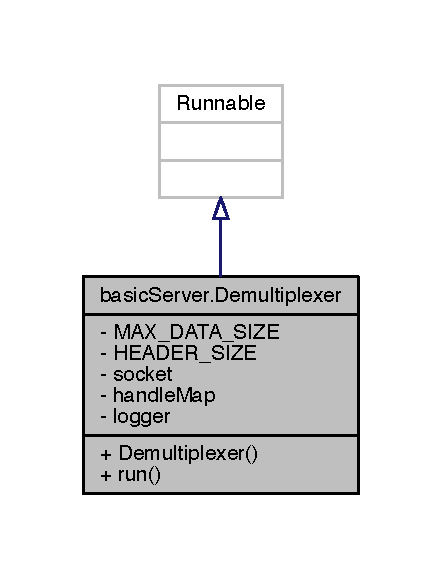
\includegraphics[width=212pt]{classbasic_server_1_1_demultiplexer__inherit__graph}
\end{center}
\end{figure}


basic\+Server.\+Demultiplexer에 대한 협력 다이어그램\+:
\nopagebreak
\begin{figure}[H]
\begin{center}
\leavevmode
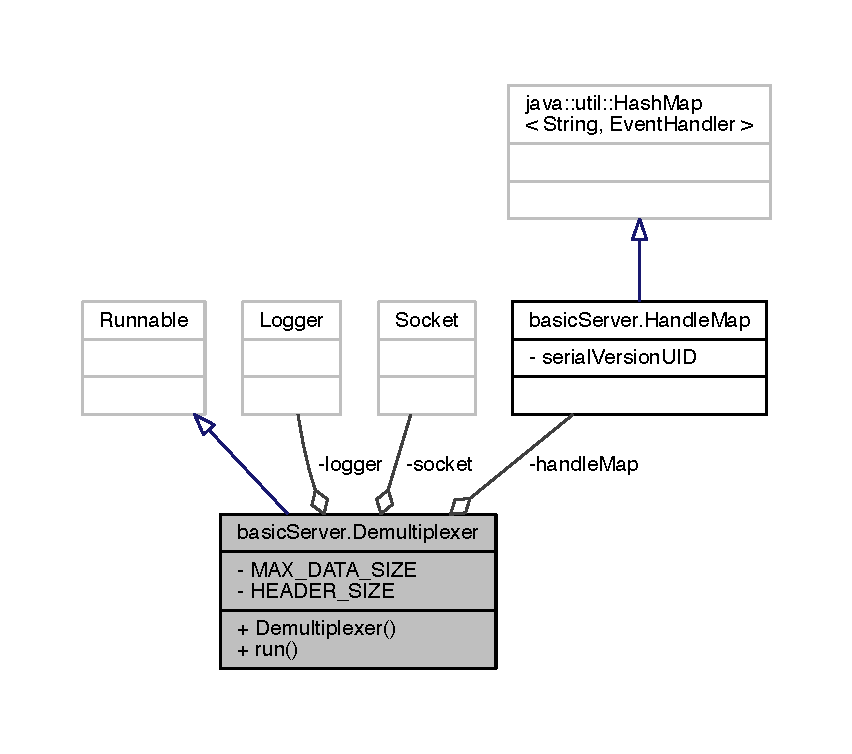
\includegraphics[width=350pt]{classbasic_server_1_1_demultiplexer__coll__graph}
\end{center}
\end{figure}
\subsection*{Public 멤버 함수}
\begin{DoxyCompactItemize}
\item 
\hyperlink{classbasic_server_1_1_demultiplexer_ab8d7da48a98765e8d5025701e1781897}{Demultiplexer} (Socket \hyperlink{classbasic_server_1_1_demultiplexer_ae73d9106d863dd9c902a2a941619056b}{socket}, \hyperlink{classbasic_server_1_1_handle_map}{Handle\+Map} \hyperlink{classbasic_server_1_1_demultiplexer_a9faf12f00a74f61936cff837b03609bd}{handle\+Map})
\item 
void \hyperlink{classbasic_server_1_1_demultiplexer_a49f039cbe9f7654b720fcd9e53a0c432}{run} ()
\end{DoxyCompactItemize}
\subsection*{Private 속성}
\begin{DoxyCompactItemize}
\item 
final int \hyperlink{classbasic_server_1_1_demultiplexer_a22d173243d9c6e9b3715330181f2d891}{M\+A\+X\+\_\+\+D\+A\+T\+A\+\_\+\+S\+I\+Z\+E} = 512 + 6
\item 
final int \hyperlink{classbasic_server_1_1_demultiplexer_a43686b9c044fc363ba7a9eae1f79120f}{H\+E\+A\+D\+E\+R\+\_\+\+S\+I\+Z\+E} = 6
\item 
Socket \hyperlink{classbasic_server_1_1_demultiplexer_ae73d9106d863dd9c902a2a941619056b}{socket}
\item 
\hyperlink{classbasic_server_1_1_handle_map}{Handle\+Map} \hyperlink{classbasic_server_1_1_demultiplexer_a9faf12f00a74f61936cff837b03609bd}{handle\+Map}
\end{DoxyCompactItemize}
\subsection*{정적 Private 속성}
\begin{DoxyCompactItemize}
\item 
static Logger \hyperlink{classbasic_server_1_1_demultiplexer_afea28eb5eb1482f56ce6b661232767b1}{logger} = Logger.\+get\+Logger(Demultiplexer.\+class.\+get\+Name())
\end{DoxyCompactItemize}


\subsection{상세한 설명}
Input Stream에서 header를 읽고 적절한 event handler를 부른다. 

\begin{DoxyDate}{날짜}
2014-\/09-\/24 
\end{DoxyDate}
\begin{DoxyAuthor}{작성자}
min 
\end{DoxyAuthor}


Demultiplexer.\+java 파일의 18 번째 라인에서 정의되었습니다.



\subsection{생성자 \& 소멸자 문서화}
\hypertarget{classbasic_server_1_1_demultiplexer_ab8d7da48a98765e8d5025701e1781897}{\index{basic\+Server\+::\+Demultiplexer@{basic\+Server\+::\+Demultiplexer}!Demultiplexer@{Demultiplexer}}
\index{Demultiplexer@{Demultiplexer}!basic\+Server\+::\+Demultiplexer@{basic\+Server\+::\+Demultiplexer}}
\subsubsection[{Demultiplexer}]{\setlength{\rightskip}{0pt plus 5cm}basic\+Server.\+Demultiplexer.\+Demultiplexer (
\begin{DoxyParamCaption}
\item[{Socket}]{socket, }
\item[{{\bf Handle\+Map}}]{handle\+Map}
\end{DoxyParamCaption}
)}}\label{classbasic_server_1_1_demultiplexer_ab8d7da48a98765e8d5025701e1781897}


Demultiplexer.\+java 파일의 27 번째 라인에서 정의되었습니다.


\begin{DoxyCode}
27                                                              \{
28         this.\hyperlink{classbasic_server_1_1_demultiplexer_ae73d9106d863dd9c902a2a941619056b}{socket} = \hyperlink{classbasic_server_1_1_demultiplexer_ae73d9106d863dd9c902a2a941619056b}{socket};
29         this.\hyperlink{classbasic_server_1_1_demultiplexer_a9faf12f00a74f61936cff837b03609bd}{handleMap} = \hyperlink{classbasic_server_1_1_demultiplexer_a9faf12f00a74f61936cff837b03609bd}{handleMap};
30     \}
\end{DoxyCode}


\subsection{멤버 함수 문서화}
\hypertarget{classbasic_server_1_1_demultiplexer_a49f039cbe9f7654b720fcd9e53a0c432}{\index{basic\+Server\+::\+Demultiplexer@{basic\+Server\+::\+Demultiplexer}!run@{run}}
\index{run@{run}!basic\+Server\+::\+Demultiplexer@{basic\+Server\+::\+Demultiplexer}}
\subsubsection[{run}]{\setlength{\rightskip}{0pt plus 5cm}void basic\+Server.\+Demultiplexer.\+run (
\begin{DoxyParamCaption}
{}
\end{DoxyParamCaption}
)}}\label{classbasic_server_1_1_demultiplexer_a49f039cbe9f7654b720fcd9e53a0c432}


Demultiplexer.\+java 파일의 33 번째 라인에서 정의되었습니다.


\begin{DoxyCode}
33                       \{
34         \textcolor{keywordflow}{try} \{
35             InputStream originalInputStream = \hyperlink{classbasic_server_1_1_demultiplexer_ae73d9106d863dd9c902a2a941619056b}{socket}.getInputStream();
36             InputStream inputStream;
37 
38             ByteArrayOutputStream byteArrayOutputStream = \textcolor{keyword}{new} ByteArrayOutputStream();
39             byte[] fullBuffer = \textcolor{keyword}{new} byte[\hyperlink{classbasic_server_1_1_demultiplexer_a22d173243d9c6e9b3715330181f2d891}{MAX\_DATA\_SIZE}];
40             byte[] headerBuffer = \textcolor{keyword}{new} byte[\hyperlink{classbasic_server_1_1_demultiplexer_a43686b9c044fc363ba7a9eae1f79120f}{HEADER\_SIZE}];
41             
42             originalInputStream.read(fullBuffer);
43             byteArrayOutputStream.write(fullBuffer);
44             
45             byteArrayOutputStream.flush();
46 
47             inputStream = \textcolor{keyword}{new} ByteArrayInputStream(byteArrayOutputStream.toByteArray()); 
48             
49             \hyperlink{classbasic_server_1_1_demultiplexer_afea28eb5eb1482f56ce6b661232767b1}{logger}.fatal(\textcolor{stringliteral}{"INPUT: "} + \textcolor{keyword}{new} String(fullBuffer));
50             
51             inputStream.read(headerBuffer);
52             String header = \textcolor{keyword}{new} String(headerBuffer);
53 
54             \hyperlink{classbasic_server_1_1_demultiplexer_a9faf12f00a74f61936cff837b03609bd}{handleMap}.get(header).handleEvent(inputStream);
55         \} \textcolor{keywordflow}{catch} (IOException e) \{
56             e.printStackTrace();
57         \}       
58     \}
\end{DoxyCode}


\subsection{멤버 데이타 문서화}
\hypertarget{classbasic_server_1_1_demultiplexer_a9faf12f00a74f61936cff837b03609bd}{\index{basic\+Server\+::\+Demultiplexer@{basic\+Server\+::\+Demultiplexer}!handle\+Map@{handle\+Map}}
\index{handle\+Map@{handle\+Map}!basic\+Server\+::\+Demultiplexer@{basic\+Server\+::\+Demultiplexer}}
\subsubsection[{handle\+Map}]{\setlength{\rightskip}{0pt plus 5cm}{\bf Handle\+Map} basic\+Server.\+Demultiplexer.\+handle\+Map\hspace{0.3cm}{\ttfamily [private]}}}\label{classbasic_server_1_1_demultiplexer_a9faf12f00a74f61936cff837b03609bd}


Demultiplexer.\+java 파일의 25 번째 라인에서 정의되었습니다.

\hypertarget{classbasic_server_1_1_demultiplexer_a43686b9c044fc363ba7a9eae1f79120f}{\index{basic\+Server\+::\+Demultiplexer@{basic\+Server\+::\+Demultiplexer}!H\+E\+A\+D\+E\+R\+\_\+\+S\+I\+Z\+E@{H\+E\+A\+D\+E\+R\+\_\+\+S\+I\+Z\+E}}
\index{H\+E\+A\+D\+E\+R\+\_\+\+S\+I\+Z\+E@{H\+E\+A\+D\+E\+R\+\_\+\+S\+I\+Z\+E}!basic\+Server\+::\+Demultiplexer@{basic\+Server\+::\+Demultiplexer}}
\subsubsection[{H\+E\+A\+D\+E\+R\+\_\+\+S\+I\+Z\+E}]{\setlength{\rightskip}{0pt plus 5cm}final int basic\+Server.\+Demultiplexer.\+H\+E\+A\+D\+E\+R\+\_\+\+S\+I\+Z\+E = 6\hspace{0.3cm}{\ttfamily [private]}}}\label{classbasic_server_1_1_demultiplexer_a43686b9c044fc363ba7a9eae1f79120f}


Demultiplexer.\+java 파일의 22 번째 라인에서 정의되었습니다.

\hypertarget{classbasic_server_1_1_demultiplexer_afea28eb5eb1482f56ce6b661232767b1}{\index{basic\+Server\+::\+Demultiplexer@{basic\+Server\+::\+Demultiplexer}!logger@{logger}}
\index{logger@{logger}!basic\+Server\+::\+Demultiplexer@{basic\+Server\+::\+Demultiplexer}}
\subsubsection[{logger}]{\setlength{\rightskip}{0pt plus 5cm}Logger basic\+Server.\+Demultiplexer.\+logger = Logger.\+get\+Logger(Demultiplexer.\+class.\+get\+Name())\hspace{0.3cm}{\ttfamily [static]}, {\ttfamily [private]}}}\label{classbasic_server_1_1_demultiplexer_afea28eb5eb1482f56ce6b661232767b1}


Demultiplexer.\+java 파일의 19 번째 라인에서 정의되었습니다.

\hypertarget{classbasic_server_1_1_demultiplexer_a22d173243d9c6e9b3715330181f2d891}{\index{basic\+Server\+::\+Demultiplexer@{basic\+Server\+::\+Demultiplexer}!M\+A\+X\+\_\+\+D\+A\+T\+A\+\_\+\+S\+I\+Z\+E@{M\+A\+X\+\_\+\+D\+A\+T\+A\+\_\+\+S\+I\+Z\+E}}
\index{M\+A\+X\+\_\+\+D\+A\+T\+A\+\_\+\+S\+I\+Z\+E@{M\+A\+X\+\_\+\+D\+A\+T\+A\+\_\+\+S\+I\+Z\+E}!basic\+Server\+::\+Demultiplexer@{basic\+Server\+::\+Demultiplexer}}
\subsubsection[{M\+A\+X\+\_\+\+D\+A\+T\+A\+\_\+\+S\+I\+Z\+E}]{\setlength{\rightskip}{0pt plus 5cm}final int basic\+Server.\+Demultiplexer.\+M\+A\+X\+\_\+\+D\+A\+T\+A\+\_\+\+S\+I\+Z\+E = 512 + 6\hspace{0.3cm}{\ttfamily [private]}}}\label{classbasic_server_1_1_demultiplexer_a22d173243d9c6e9b3715330181f2d891}


Demultiplexer.\+java 파일의 21 번째 라인에서 정의되었습니다.

\hypertarget{classbasic_server_1_1_demultiplexer_ae73d9106d863dd9c902a2a941619056b}{\index{basic\+Server\+::\+Demultiplexer@{basic\+Server\+::\+Demultiplexer}!socket@{socket}}
\index{socket@{socket}!basic\+Server\+::\+Demultiplexer@{basic\+Server\+::\+Demultiplexer}}
\subsubsection[{socket}]{\setlength{\rightskip}{0pt plus 5cm}Socket basic\+Server.\+Demultiplexer.\+socket\hspace{0.3cm}{\ttfamily [private]}}}\label{classbasic_server_1_1_demultiplexer_ae73d9106d863dd9c902a2a941619056b}


Demultiplexer.\+java 파일의 24 번째 라인에서 정의되었습니다.



이 클래스에 대한 문서화 페이지는 다음의 파일로부터 생성되었습니다.\+:\begin{DoxyCompactItemize}
\item 
src/basic\+Server/\hyperlink{_demultiplexer_8java}{Demultiplexer.\+java}\end{DoxyCompactItemize}

\hypertarget{interfacebasic_server_1_1_dispatcher}{\section{basic\+Server.\+Dispatcher 인터페이스 참조}
\label{interfacebasic_server_1_1_dispatcher}\index{basic\+Server.\+Dispatcher@{basic\+Server.\+Dispatcher}}
}


dispatcher의 D\+I를 위한 인터페이스  




basic\+Server.\+Dispatcher에 대한 상속 다이어그램 \+: 
\nopagebreak
\begin{figure}[H]
\begin{center}
\leavevmode
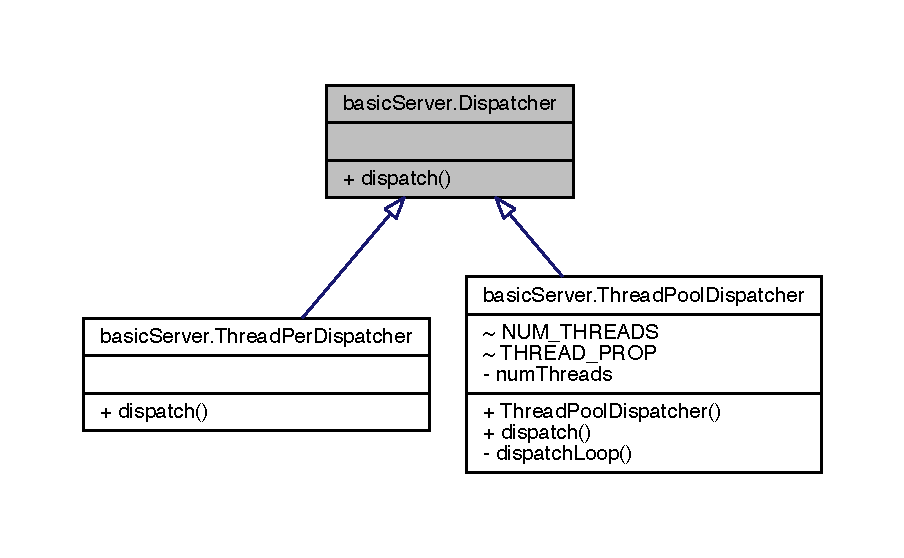
\includegraphics[width=350pt]{interfacebasic_server_1_1_dispatcher__inherit__graph}
\end{center}
\end{figure}


basic\+Server.\+Dispatcher에 대한 협력 다이어그램\+:\nopagebreak
\begin{figure}[H]
\begin{center}
\leavevmode
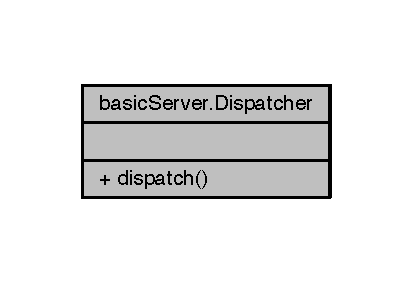
\includegraphics[width=198pt]{interfacebasic_server_1_1_dispatcher__coll__graph}
\end{center}
\end{figure}
\subsection*{Public 멤버 함수}
\begin{DoxyCompactItemize}
\item 
void \hyperlink{interfacebasic_server_1_1_dispatcher_a9a8d3e47b27a6161f8f39bf63fa9e198}{dispatch} (Server\+Socket server\+Socket, \hyperlink{classbasic_server_1_1_handle_map}{Handle\+Map} handle\+Map)
\end{DoxyCompactItemize}


\subsection{상세한 설명}
dispatcher의 D\+I를 위한 인터페이스 

\begin{DoxyDate}{날짜}
2014-\/09-\/24 
\end{DoxyDate}
\begin{DoxyAuthor}{작성자}
min 
\end{DoxyAuthor}


Dispatcher.\+java 파일의 11 번째 라인에서 정의되었습니다.



\subsection{멤버 함수 문서화}
\hypertarget{interfacebasic_server_1_1_dispatcher_a9a8d3e47b27a6161f8f39bf63fa9e198}{\index{basic\+Server\+::\+Dispatcher@{basic\+Server\+::\+Dispatcher}!dispatch@{dispatch}}
\index{dispatch@{dispatch}!basic\+Server\+::\+Dispatcher@{basic\+Server\+::\+Dispatcher}}
\subsubsection[{dispatch}]{\setlength{\rightskip}{0pt plus 5cm}void basic\+Server.\+Dispatcher.\+dispatch (
\begin{DoxyParamCaption}
\item[{Server\+Socket}]{server\+Socket, }
\item[{{\bf Handle\+Map}}]{handle\+Map}
\end{DoxyParamCaption}
)}}\label{interfacebasic_server_1_1_dispatcher_a9a8d3e47b27a6161f8f39bf63fa9e198}


\hyperlink{classbasic_server_1_1_thread_per_dispatcher_af7be4592fa9f81c011985b4e0c0c3b2a}{basic\+Server.\+Thread\+Per\+Dispatcher}에서 구현되었습니다.



이 인터페이스에 대한 문서화 페이지는 다음의 파일로부터 생성되었습니다.\+:\begin{DoxyCompactItemize}
\item 
src/basic\+Server/\hyperlink{_dispatcher_8java}{Dispatcher.\+java}\end{DoxyCompactItemize}

\hypertarget{interfaceevent_handler_1_1_event_handler}{\section{event\+Handler.\+Event\+Handler 인터페이스 참조}
\label{interfaceevent_handler_1_1_event_handler}\index{event\+Handler.\+Event\+Handler@{event\+Handler.\+Event\+Handler}}
}


event handler의 메소드를 정의한 interface.  




event\+Handler.\+Event\+Handler에 대한 상속 다이어그램 \+: 
\nopagebreak
\begin{figure}[H]
\begin{center}
\leavevmode
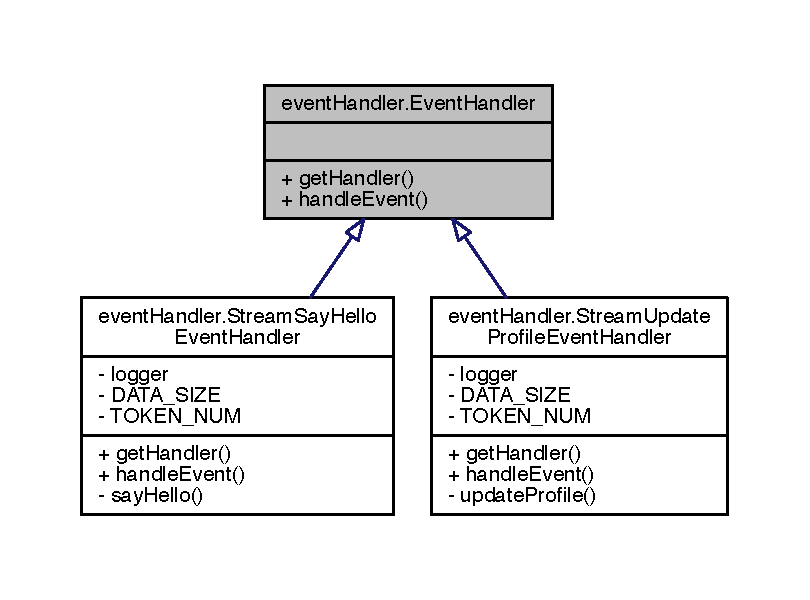
\includegraphics[width=350pt]{interfaceevent_handler_1_1_event_handler__inherit__graph}
\end{center}
\end{figure}


event\+Handler.\+Event\+Handler에 대한 협력 다이어그램\+:\nopagebreak
\begin{figure}[H]
\begin{center}
\leavevmode
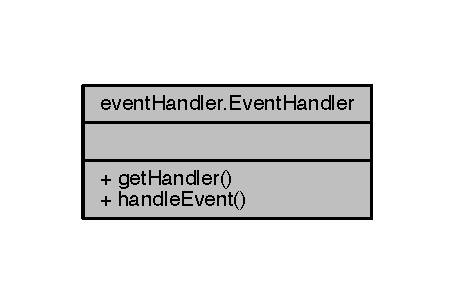
\includegraphics[width=218pt]{interfaceevent_handler_1_1_event_handler__coll__graph}
\end{center}
\end{figure}
\subsection*{Public 멤버 함수}
\begin{DoxyCompactItemize}
\item 
String \hyperlink{interfaceevent_handler_1_1_event_handler_ada178635174014bad23584547462ac03}{get\+Handler} ()
\item 
void \hyperlink{interfaceevent_handler_1_1_event_handler_a4036ea3f27edd7df0caa57f42db27eed}{handle\+Event} (Input\+Stream input\+Stream)
\end{DoxyCompactItemize}


\subsection{상세한 설명}
event handler의 메소드를 정의한 interface. 

\begin{DoxyDate}{날짜}
2014-\/09-\/24 
\end{DoxyDate}
\begin{DoxyAuthor}{작성자}
min 
\end{DoxyAuthor}


Event\+Handler.\+java 파일의 11 번째 라인에서 정의되었습니다.



\subsection{멤버 함수 문서화}
\hypertarget{interfaceevent_handler_1_1_event_handler_ada178635174014bad23584547462ac03}{\index{event\+Handler\+::\+Event\+Handler@{event\+Handler\+::\+Event\+Handler}!get\+Handler@{get\+Handler}}
\index{get\+Handler@{get\+Handler}!event\+Handler\+::\+Event\+Handler@{event\+Handler\+::\+Event\+Handler}}
\subsubsection[{get\+Handler}]{\setlength{\rightskip}{0pt plus 5cm}String event\+Handler.\+Event\+Handler.\+get\+Handler (
\begin{DoxyParamCaption}
{}
\end{DoxyParamCaption}
)}}\label{interfaceevent_handler_1_1_event_handler_ada178635174014bad23584547462ac03}


\hyperlink{classevent_handler_1_1_stream_say_hello_event_handler_a2ff06320bb8ddd881d147d31a46d365b}{event\+Handler.\+Stream\+Say\+Hello\+Event\+Handler}, \hyperlink{classevent_handler_1_1_stream_update_profile_event_handler_a24bf455a312c225975d472516b4bb6f9}{event\+Handler.\+Stream\+Update\+Profile\+Event\+Handler}에서 구현되었습니다.



이 함수를 호출하는 함수들에 대한 그래프입니다.\+:\nopagebreak
\begin{figure}[H]
\begin{center}
\leavevmode
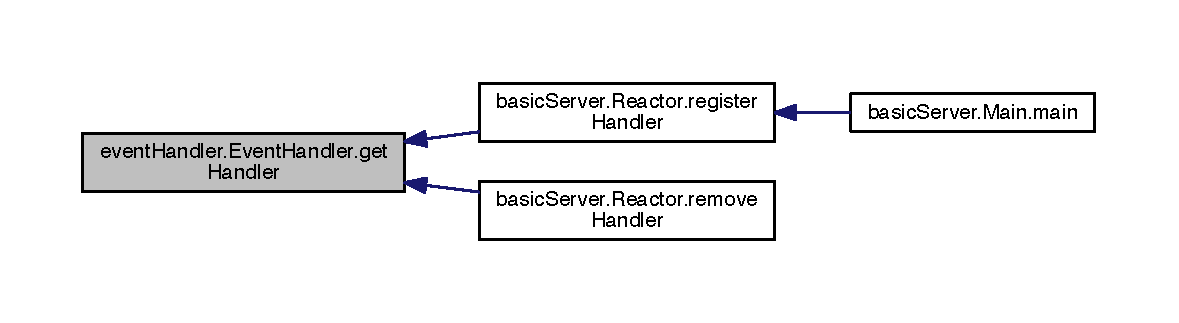
\includegraphics[width=350pt]{interfaceevent_handler_1_1_event_handler_ada178635174014bad23584547462ac03_icgraph}
\end{center}
\end{figure}


\hypertarget{interfaceevent_handler_1_1_event_handler_a4036ea3f27edd7df0caa57f42db27eed}{\index{event\+Handler\+::\+Event\+Handler@{event\+Handler\+::\+Event\+Handler}!handle\+Event@{handle\+Event}}
\index{handle\+Event@{handle\+Event}!event\+Handler\+::\+Event\+Handler@{event\+Handler\+::\+Event\+Handler}}
\subsubsection[{handle\+Event}]{\setlength{\rightskip}{0pt plus 5cm}void event\+Handler.\+Event\+Handler.\+handle\+Event (
\begin{DoxyParamCaption}
\item[{Input\+Stream}]{input\+Stream}
\end{DoxyParamCaption}
)}}\label{interfaceevent_handler_1_1_event_handler_a4036ea3f27edd7df0caa57f42db27eed}


\hyperlink{classevent_handler_1_1_stream_say_hello_event_handler_a859dc382ae8a35257af2149a9ed1c6b8}{event\+Handler.\+Stream\+Say\+Hello\+Event\+Handler}, \hyperlink{classevent_handler_1_1_stream_update_profile_event_handler_a96b3a510c642a6848cff0afce54b7d8e}{event\+Handler.\+Stream\+Update\+Profile\+Event\+Handler}에서 구현되었습니다.



이 인터페이스에 대한 문서화 페이지는 다음의 파일로부터 생성되었습니다.\+:\begin{DoxyCompactItemize}
\item 
src/event\+Handler/\hyperlink{_event_handler_8java}{Event\+Handler.\+java}\end{DoxyCompactItemize}

\hypertarget{classbasic_server_1_1_handle_map}{\section{basic\+Server.\+Handle\+Map 클래스 참조}
\label{classbasic_server_1_1_handle_map}\index{basic\+Server.\+Handle\+Map@{basic\+Server.\+Handle\+Map}}
}


header와 그에 대응하는 event handler를 기억함  




basic\+Server.\+Handle\+Map에 대한 상속 다이어그램 \+: \nopagebreak
\begin{figure}[H]
\begin{center}
\leavevmode
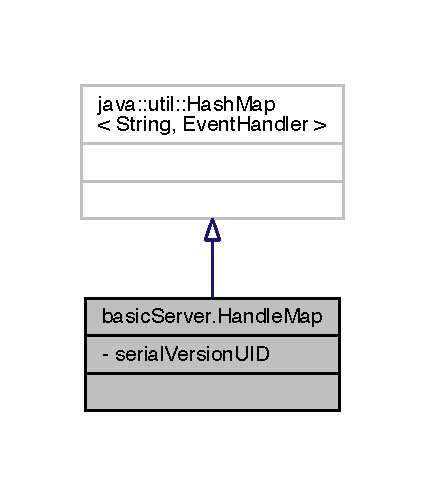
\includegraphics[width=204pt]{classbasic_server_1_1_handle_map__inherit__graph}
\end{center}
\end{figure}


basic\+Server.\+Handle\+Map에 대한 협력 다이어그램\+:\nopagebreak
\begin{figure}[H]
\begin{center}
\leavevmode
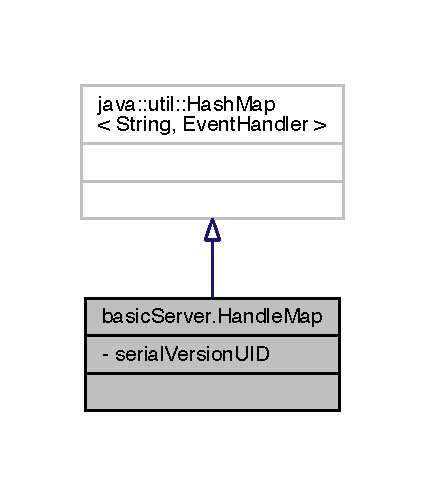
\includegraphics[width=204pt]{classbasic_server_1_1_handle_map__coll__graph}
\end{center}
\end{figure}
\subsection*{정적 Private 속성}
\begin{DoxyCompactItemize}
\item 
static final long \hyperlink{classbasic_server_1_1_handle_map_ac3933c5d00781beb6cf93b4056f71cd4}{serial\+Version\+U\+I\+D} = 1\+L
\end{DoxyCompactItemize}


\subsection{상세한 설명}
header와 그에 대응하는 event handler를 기억함 

\begin{DoxyDate}{날짜}
2014-\/09-\/24 
\end{DoxyDate}
\begin{DoxyAuthor}{작성자}
min 
\end{DoxyAuthor}


Handle\+Map.\+java 파일의 13 번째 라인에서 정의되었습니다.



\subsection{멤버 데이타 문서화}
\hypertarget{classbasic_server_1_1_handle_map_ac3933c5d00781beb6cf93b4056f71cd4}{\index{basic\+Server\+::\+Handle\+Map@{basic\+Server\+::\+Handle\+Map}!serial\+Version\+U\+I\+D@{serial\+Version\+U\+I\+D}}
\index{serial\+Version\+U\+I\+D@{serial\+Version\+U\+I\+D}!basic\+Server\+::\+Handle\+Map@{basic\+Server\+::\+Handle\+Map}}
\subsubsection[{serial\+Version\+U\+I\+D}]{\setlength{\rightskip}{0pt plus 5cm}final long basic\+Server.\+Handle\+Map.\+serial\+Version\+U\+I\+D = 1\+L\hspace{0.3cm}{\ttfamily [static]}, {\ttfamily [private]}}}\label{classbasic_server_1_1_handle_map_ac3933c5d00781beb6cf93b4056f71cd4}


Handle\+Map.\+java 파일의 14 번째 라인에서 정의되었습니다.



이 클래스에 대한 문서화 페이지는 다음의 파일로부터 생성되었습니다.\+:\begin{DoxyCompactItemize}
\item 
src/basic\+Server/\hyperlink{_handle_map_8java}{Handle\+Map.\+java}\end{DoxyCompactItemize}

\hypertarget{classbasic_server_1_1_main}{\section{basic\+Server.\+Main 클래스 참조}
\label{classbasic_server_1_1_main}\index{basic\+Server.\+Main@{basic\+Server.\+Main}}
}


main함수를 갖고 있다. reactor를 new하고 실행시킨다.  




basic\+Server.\+Main에 대한 협력 다이어그램\+:\nopagebreak
\begin{figure}[H]
\begin{center}
\leavevmode
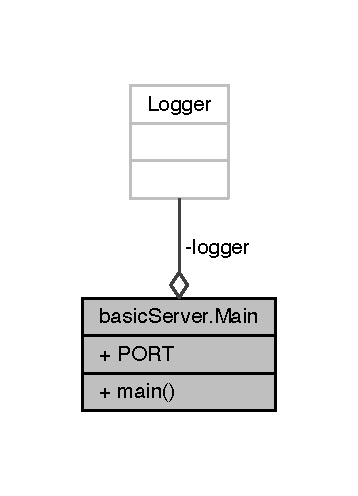
\includegraphics[width=172pt]{classbasic_server_1_1_main__coll__graph}
\end{center}
\end{figure}
\subsection*{정적 Public 멤버 함수}
\begin{DoxyCompactItemize}
\item 
static void \hyperlink{classbasic_server_1_1_main_a0c7ee477ff533ef286ecf5a95148eda8}{main} (String\mbox{[}$\,$\mbox{]} args)
\end{DoxyCompactItemize}
\subsection*{정적 Public 속성}
\begin{DoxyCompactItemize}
\item 
static final int \hyperlink{classbasic_server_1_1_main_af83ee27a3ec7ae49bcfed0bc78bd32ca}{P\+O\+R\+T} = 5000
\end{DoxyCompactItemize}
\subsection*{정적 Private 속성}
\begin{DoxyCompactItemize}
\item 
static Logger \hyperlink{classbasic_server_1_1_main_a41d7399aaeba39a260abea976c89600b}{logger} = Logger.\+get\+Logger(Main.\+class.\+get\+Name())
\end{DoxyCompactItemize}


\subsection{상세한 설명}
main함수를 갖고 있다. reactor를 new하고 실행시킨다. 

\begin{DoxyDate}{날짜}
2014-\/09-\/24 
\end{DoxyDate}
\begin{DoxyAuthor}{작성자}
min 
\end{DoxyAuthor}


Main.\+java 파일의 14 번째 라인에서 정의되었습니다.



\subsection{멤버 함수 문서화}
\hypertarget{classbasic_server_1_1_main_a0c7ee477ff533ef286ecf5a95148eda8}{\index{basic\+Server\+::\+Main@{basic\+Server\+::\+Main}!main@{main}}
\index{main@{main}!basic\+Server\+::\+Main@{basic\+Server\+::\+Main}}
\subsubsection[{main}]{\setlength{\rightskip}{0pt plus 5cm}static void basic\+Server.\+Main.\+main (
\begin{DoxyParamCaption}
\item[{String\mbox{[}$\,$\mbox{]}}]{args}
\end{DoxyParamCaption}
)\hspace{0.3cm}{\ttfamily [static]}}}\label{classbasic_server_1_1_main_a0c7ee477ff533ef286ecf5a95148eda8}


Main.\+java 파일의 19 번째 라인에서 정의되었습니다.


\begin{DoxyCode}
19                                            \{
20         System.out.println(\textcolor{stringliteral}{"SERVER START at PORT: "} + \hyperlink{classbasic_server_1_1_main_af83ee27a3ec7ae49bcfed0bc78bd32ca}{PORT} + \textcolor{stringliteral}{"!"});
21         
22         \textcolor{comment}{// Init Test}
23         \textcolor{comment}{//logger.fatal("log4j: logger.fatal()");}
24         \textcolor{comment}{//logger.error("log4j: logger.error()");}
25         \textcolor{comment}{//logger.warn("log4j: logger.warn()");}
26         \textcolor{comment}{//logger.info("log4j: logger.info()");}
27         \textcolor{comment}{//logger.debug("log4j: logger.debug()");}
28         \textcolor{comment}{//logger.trace("log4j: logger.trace()");}
29 
30         Reactor reactor = \textcolor{keyword}{new} Reactor(\hyperlink{classbasic_server_1_1_main_af83ee27a3ec7ae49bcfed0bc78bd32ca}{PORT});
31 
32         reactor.registerHandler(\textcolor{keyword}{new} StreamSayHelloEventHandler());
33         reactor.registerHandler(\textcolor{keyword}{new} StreamUpdateProfileEventHandler());
34 
35         reactor.startServer();
36     \}
\end{DoxyCode}


이 함수 내부에서 호출하는 함수들에 대한 그래프입니다.\+:\nopagebreak
\begin{figure}[H]
\begin{center}
\leavevmode
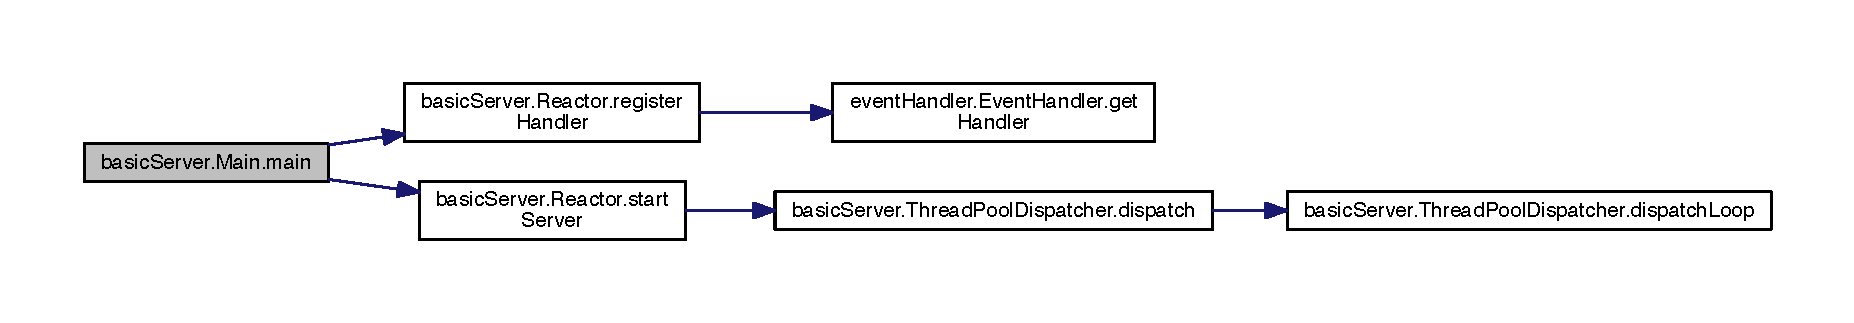
\includegraphics[width=350pt]{classbasic_server_1_1_main_a0c7ee477ff533ef286ecf5a95148eda8_cgraph}
\end{center}
\end{figure}




\subsection{멤버 데이타 문서화}
\hypertarget{classbasic_server_1_1_main_a41d7399aaeba39a260abea976c89600b}{\index{basic\+Server\+::\+Main@{basic\+Server\+::\+Main}!logger@{logger}}
\index{logger@{logger}!basic\+Server\+::\+Main@{basic\+Server\+::\+Main}}
\subsubsection[{logger}]{\setlength{\rightskip}{0pt plus 5cm}Logger basic\+Server.\+Main.\+logger = Logger.\+get\+Logger(Main.\+class.\+get\+Name())\hspace{0.3cm}{\ttfamily [static]}, {\ttfamily [private]}}}\label{classbasic_server_1_1_main_a41d7399aaeba39a260abea976c89600b}


Main.\+java 파일의 15 번째 라인에서 정의되었습니다.

\hypertarget{classbasic_server_1_1_main_af83ee27a3ec7ae49bcfed0bc78bd32ca}{\index{basic\+Server\+::\+Main@{basic\+Server\+::\+Main}!P\+O\+R\+T@{P\+O\+R\+T}}
\index{P\+O\+R\+T@{P\+O\+R\+T}!basic\+Server\+::\+Main@{basic\+Server\+::\+Main}}
\subsubsection[{P\+O\+R\+T}]{\setlength{\rightskip}{0pt plus 5cm}final int basic\+Server.\+Main.\+P\+O\+R\+T = 5000\hspace{0.3cm}{\ttfamily [static]}}}\label{classbasic_server_1_1_main_af83ee27a3ec7ae49bcfed0bc78bd32ca}


Main.\+java 파일의 17 번째 라인에서 정의되었습니다.



이 클래스에 대한 문서화 페이지는 다음의 파일로부터 생성되었습니다.\+:\begin{DoxyCompactItemize}
\item 
src/basic\+Server/\hyperlink{_main_8java}{Main.\+java}\end{DoxyCompactItemize}

\hypertarget{classbasic_server_1_1_reactor}{\section{basic\+Server.\+Reactor 클래스 참조}
\label{classbasic_server_1_1_reactor}\index{basic\+Server.\+Reactor@{basic\+Server.\+Reactor}}
}


dispatcher 관리, header와 대응되는 event handler를 관리.  




basic\+Server.\+Reactor에 대한 협력 다이어그램\+:
\nopagebreak
\begin{figure}[H]
\begin{center}
\leavevmode
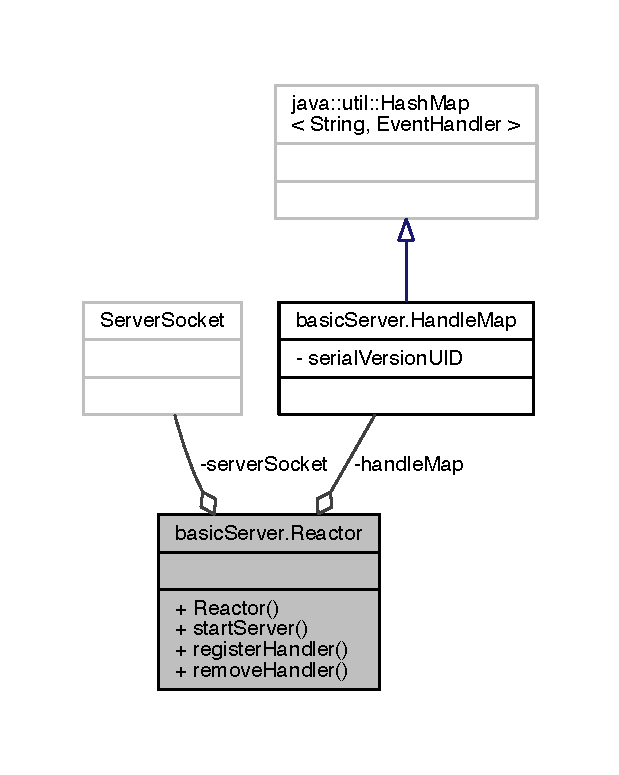
\includegraphics[width=297pt]{classbasic_server_1_1_reactor__coll__graph}
\end{center}
\end{figure}
\subsection*{Public 멤버 함수}
\begin{DoxyCompactItemize}
\item 
\hyperlink{classbasic_server_1_1_reactor_ad31c6a01771438f1f124eba778e49c0a}{Reactor} (int port)
\item 
void \hyperlink{classbasic_server_1_1_reactor_aaa28ae533a17acacc0acb5a7161c84e5}{start\+Server} ()
\item 
void \hyperlink{classbasic_server_1_1_reactor_ab74b6a96ff989298eb36a1cf3fd0e69f}{register\+Handler} (\hyperlink{interfaceevent_handler_1_1_event_handler}{Event\+Handler} handler)
\item 
void \hyperlink{classbasic_server_1_1_reactor_ab50f8b7b6adf4b18ccca715fa2ca8182}{remove\+Handler} (\hyperlink{interfaceevent_handler_1_1_event_handler}{Event\+Handler} handler)
\end{DoxyCompactItemize}
\subsection*{Private 속성}
\begin{DoxyCompactItemize}
\item 
Server\+Socket \hyperlink{classbasic_server_1_1_reactor_a2ddae2bb37e01fa74cfdd54b02ad00d0}{server\+Socket}
\item 
\hyperlink{classbasic_server_1_1_handle_map}{Handle\+Map} \hyperlink{classbasic_server_1_1_reactor_a74841c32eee00227bbd43e8d016aad20}{handle\+Map}
\end{DoxyCompactItemize}


\subsection{상세한 설명}
dispatcher 관리, header와 대응되는 event handler를 관리. 

\begin{DoxyDate}{날짜}
2014-\/09-\/24 
\end{DoxyDate}
\begin{DoxyAuthor}{작성자}
min 
\end{DoxyAuthor}


Reactor.\+java 파일의 14 번째 라인에서 정의되었습니다.



\subsection{생성자 \& 소멸자 문서화}
\hypertarget{classbasic_server_1_1_reactor_ad31c6a01771438f1f124eba778e49c0a}{\index{basic\+Server\+::\+Reactor@{basic\+Server\+::\+Reactor}!Reactor@{Reactor}}
\index{Reactor@{Reactor}!basic\+Server\+::\+Reactor@{basic\+Server\+::\+Reactor}}
\subsubsection[{Reactor}]{\setlength{\rightskip}{0pt plus 5cm}basic\+Server.\+Reactor.\+Reactor (
\begin{DoxyParamCaption}
\item[{int}]{port}
\end{DoxyParamCaption}
)}}\label{classbasic_server_1_1_reactor_ad31c6a01771438f1f124eba778e49c0a}


Reactor.\+java 파일의 18 번째 라인에서 정의되었습니다.


\begin{DoxyCode}
18                              \{
19         \hyperlink{classbasic_server_1_1_reactor_a74841c32eee00227bbd43e8d016aad20}{handleMap} = \textcolor{keyword}{new} HandleMap();
20 
21         \textcolor{keywordflow}{try} \{
22             \hyperlink{classbasic_server_1_1_reactor_a2ddae2bb37e01fa74cfdd54b02ad00d0}{serverSocket} = \textcolor{keyword}{new} ServerSocket(port);
23         \} \textcolor{keywordflow}{catch} (IOException e) \{
24             e.printStackTrace();
25         \}
26     \}
\end{DoxyCode}


\subsection{멤버 함수 문서화}
\hypertarget{classbasic_server_1_1_reactor_ab74b6a96ff989298eb36a1cf3fd0e69f}{\index{basic\+Server\+::\+Reactor@{basic\+Server\+::\+Reactor}!register\+Handler@{register\+Handler}}
\index{register\+Handler@{register\+Handler}!basic\+Server\+::\+Reactor@{basic\+Server\+::\+Reactor}}
\subsubsection[{register\+Handler}]{\setlength{\rightskip}{0pt plus 5cm}void basic\+Server.\+Reactor.\+register\+Handler (
\begin{DoxyParamCaption}
\item[{{\bf Event\+Handler}}]{handler}
\end{DoxyParamCaption}
)}}\label{classbasic_server_1_1_reactor_ab74b6a96ff989298eb36a1cf3fd0e69f}


Reactor.\+java 파일의 34 번째 라인에서 정의되었습니다.


\begin{DoxyCode}
34                                                       \{
35         \hyperlink{classbasic_server_1_1_reactor_a74841c32eee00227bbd43e8d016aad20}{handleMap}.put(handler.getHandler(), handler);
36     \}
\end{DoxyCode}


이 함수 내부에서 호출하는 함수들에 대한 그래프입니다.\+:\nopagebreak
\begin{figure}[H]
\begin{center}
\leavevmode
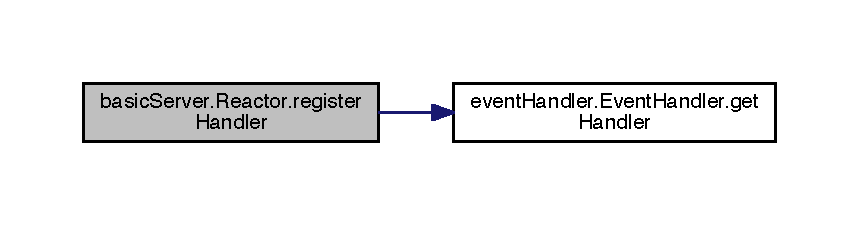
\includegraphics[width=350pt]{classbasic_server_1_1_reactor_ab74b6a96ff989298eb36a1cf3fd0e69f_cgraph}
\end{center}
\end{figure}




이 함수를 호출하는 함수들에 대한 그래프입니다.\+:\nopagebreak
\begin{figure}[H]
\begin{center}
\leavevmode
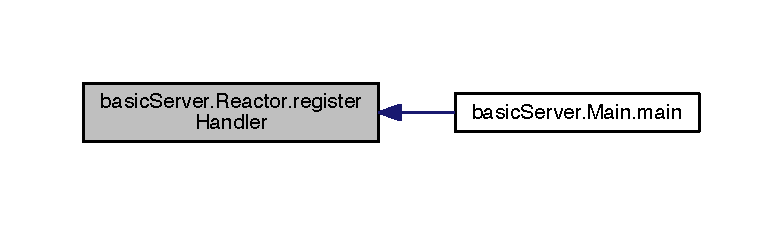
\includegraphics[width=350pt]{classbasic_server_1_1_reactor_ab74b6a96ff989298eb36a1cf3fd0e69f_icgraph}
\end{center}
\end{figure}


\hypertarget{classbasic_server_1_1_reactor_ab50f8b7b6adf4b18ccca715fa2ca8182}{\index{basic\+Server\+::\+Reactor@{basic\+Server\+::\+Reactor}!remove\+Handler@{remove\+Handler}}
\index{remove\+Handler@{remove\+Handler}!basic\+Server\+::\+Reactor@{basic\+Server\+::\+Reactor}}
\subsubsection[{remove\+Handler}]{\setlength{\rightskip}{0pt plus 5cm}void basic\+Server.\+Reactor.\+remove\+Handler (
\begin{DoxyParamCaption}
\item[{{\bf Event\+Handler}}]{handler}
\end{DoxyParamCaption}
)}}\label{classbasic_server_1_1_reactor_ab50f8b7b6adf4b18ccca715fa2ca8182}


Reactor.\+java 파일의 38 번째 라인에서 정의되었습니다.


\begin{DoxyCode}
38                                                     \{
39         \hyperlink{classbasic_server_1_1_reactor_a74841c32eee00227bbd43e8d016aad20}{handleMap}.remove(handler.getHandler());
40     \}
\end{DoxyCode}


이 함수 내부에서 호출하는 함수들에 대한 그래프입니다.\+:\nopagebreak
\begin{figure}[H]
\begin{center}
\leavevmode
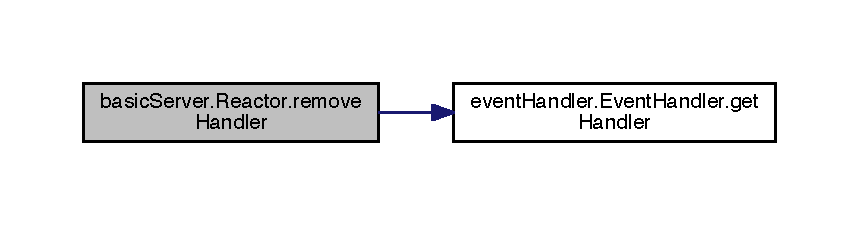
\includegraphics[width=350pt]{classbasic_server_1_1_reactor_ab50f8b7b6adf4b18ccca715fa2ca8182_cgraph}
\end{center}
\end{figure}


\hypertarget{classbasic_server_1_1_reactor_aaa28ae533a17acacc0acb5a7161c84e5}{\index{basic\+Server\+::\+Reactor@{basic\+Server\+::\+Reactor}!start\+Server@{start\+Server}}
\index{start\+Server@{start\+Server}!basic\+Server\+::\+Reactor@{basic\+Server\+::\+Reactor}}
\subsubsection[{start\+Server}]{\setlength{\rightskip}{0pt plus 5cm}void basic\+Server.\+Reactor.\+start\+Server (
\begin{DoxyParamCaption}
{}
\end{DoxyParamCaption}
)}}\label{classbasic_server_1_1_reactor_aaa28ae533a17acacc0acb5a7161c84e5}


Reactor.\+java 파일의 28 번째 라인에서 정의되었습니다.


\begin{DoxyCode}
28                               \{
29         \textcolor{comment}{// ThreadPerDispatcher dispatcher = new ThreadPerDispatcher();}
30         ThreadPoolDispatcher dispatcher = \textcolor{keyword}{new} ThreadPoolDispatcher();
31         dispatcher.dispatch(\hyperlink{classbasic_server_1_1_reactor_a2ddae2bb37e01fa74cfdd54b02ad00d0}{serverSocket}, \hyperlink{classbasic_server_1_1_reactor_a74841c32eee00227bbd43e8d016aad20}{handleMap});
32     \}
\end{DoxyCode}


이 함수 내부에서 호출하는 함수들에 대한 그래프입니다.\+:\nopagebreak
\begin{figure}[H]
\begin{center}
\leavevmode
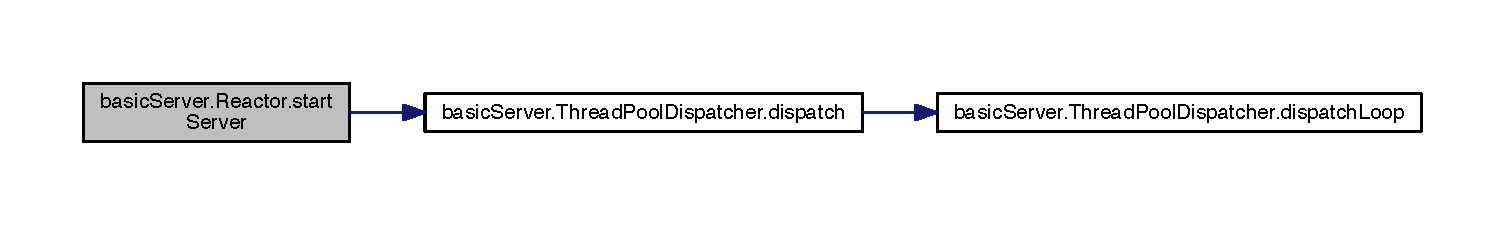
\includegraphics[width=350pt]{classbasic_server_1_1_reactor_aaa28ae533a17acacc0acb5a7161c84e5_cgraph}
\end{center}
\end{figure}




이 함수를 호출하는 함수들에 대한 그래프입니다.\+:\nopagebreak
\begin{figure}[H]
\begin{center}
\leavevmode
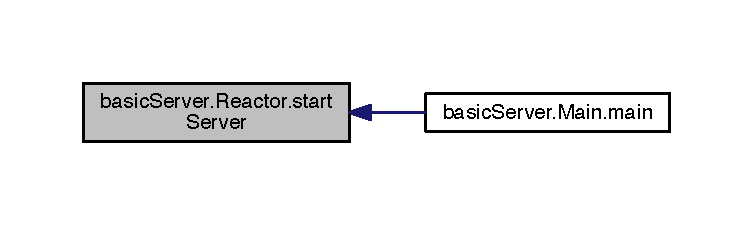
\includegraphics[width=350pt]{classbasic_server_1_1_reactor_aaa28ae533a17acacc0acb5a7161c84e5_icgraph}
\end{center}
\end{figure}




\subsection{멤버 데이타 문서화}
\hypertarget{classbasic_server_1_1_reactor_a74841c32eee00227bbd43e8d016aad20}{\index{basic\+Server\+::\+Reactor@{basic\+Server\+::\+Reactor}!handle\+Map@{handle\+Map}}
\index{handle\+Map@{handle\+Map}!basic\+Server\+::\+Reactor@{basic\+Server\+::\+Reactor}}
\subsubsection[{handle\+Map}]{\setlength{\rightskip}{0pt plus 5cm}{\bf Handle\+Map} basic\+Server.\+Reactor.\+handle\+Map\hspace{0.3cm}{\ttfamily [private]}}}\label{classbasic_server_1_1_reactor_a74841c32eee00227bbd43e8d016aad20}


Reactor.\+java 파일의 16 번째 라인에서 정의되었습니다.

\hypertarget{classbasic_server_1_1_reactor_a2ddae2bb37e01fa74cfdd54b02ad00d0}{\index{basic\+Server\+::\+Reactor@{basic\+Server\+::\+Reactor}!server\+Socket@{server\+Socket}}
\index{server\+Socket@{server\+Socket}!basic\+Server\+::\+Reactor@{basic\+Server\+::\+Reactor}}
\subsubsection[{server\+Socket}]{\setlength{\rightskip}{0pt plus 5cm}Server\+Socket basic\+Server.\+Reactor.\+server\+Socket\hspace{0.3cm}{\ttfamily [private]}}}\label{classbasic_server_1_1_reactor_a2ddae2bb37e01fa74cfdd54b02ad00d0}


Reactor.\+java 파일의 15 번째 라인에서 정의되었습니다.



이 클래스에 대한 문서화 페이지는 다음의 파일로부터 생성되었습니다.\+:\begin{DoxyCompactItemize}
\item 
src/basic\+Server/\hyperlink{_reactor_8java}{Reactor.\+java}\end{DoxyCompactItemize}

\hypertarget{classevent_handler_1_1_stream_say_hello_event_handler}{\section{event\+Handler.\+Stream\+Say\+Hello\+Event\+Handler 클래스 참조}
\label{classevent_handler_1_1_stream_say_hello_event_handler}\index{event\+Handler.\+Stream\+Say\+Hello\+Event\+Handler@{event\+Handler.\+Stream\+Say\+Hello\+Event\+Handler}}
}


0x5001 헤더를 받았을 때 실행되는 event handler. \hyperlink{classevent_handler_1_1_stream_say_hello_event_handler_a6af4d6b8a6ed973d984a2eea55e405bc}{say\+Hello()}를 갖고 있다.  




event\+Handler.\+Stream\+Say\+Hello\+Event\+Handler에 대한 상속 다이어그램 \+: 
\nopagebreak
\begin{figure}[H]
\begin{center}
\leavevmode
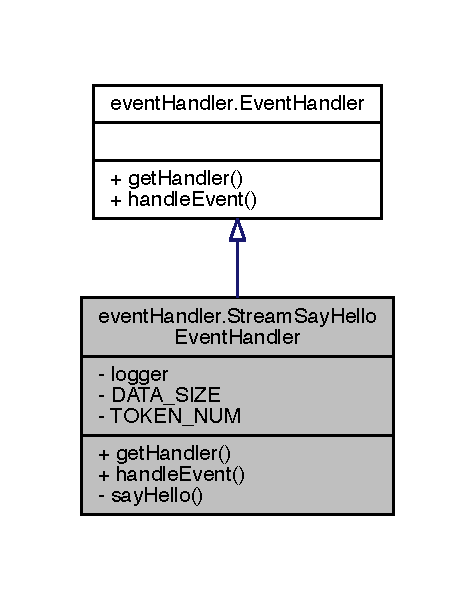
\includegraphics[width=228pt]{classevent_handler_1_1_stream_say_hello_event_handler__inherit__graph}
\end{center}
\end{figure}


event\+Handler.\+Stream\+Say\+Hello\+Event\+Handler에 대한 협력 다이어그램\+:
\nopagebreak
\begin{figure}[H]
\begin{center}
\leavevmode
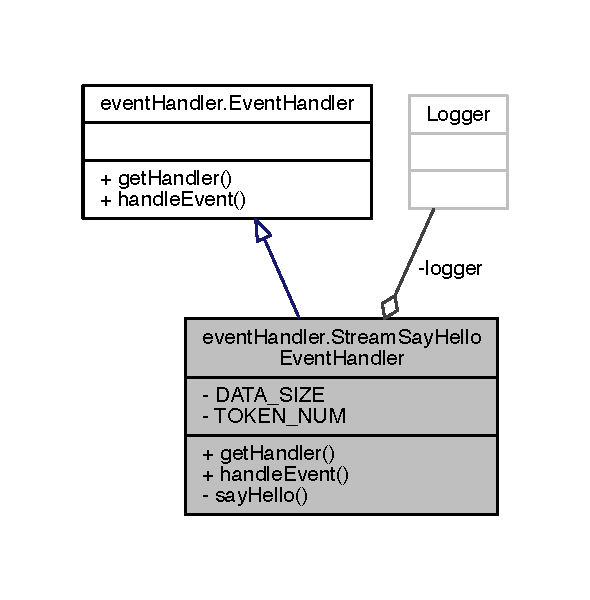
\includegraphics[width=283pt]{classevent_handler_1_1_stream_say_hello_event_handler__coll__graph}
\end{center}
\end{figure}
\subsection*{Public 멤버 함수}
\begin{DoxyCompactItemize}
\item 
String \hyperlink{classevent_handler_1_1_stream_say_hello_event_handler_a2ff06320bb8ddd881d147d31a46d365b}{get\+Handler} ()
\item 
void \hyperlink{classevent_handler_1_1_stream_say_hello_event_handler_a859dc382ae8a35257af2149a9ed1c6b8}{handle\+Event} (Input\+Stream input\+Stream)
\end{DoxyCompactItemize}
\subsection*{Private 멤버 함수}
\begin{DoxyCompactItemize}
\item 
void \hyperlink{classevent_handler_1_1_stream_say_hello_event_handler_a6af4d6b8a6ed973d984a2eea55e405bc}{say\+Hello} (String\mbox{[}$\,$\mbox{]} params)
\end{DoxyCompactItemize}
\subsection*{정적 Private 속성}
\begin{DoxyCompactItemize}
\item 
static Logger \hyperlink{classevent_handler_1_1_stream_say_hello_event_handler_a9ce34e287f4621a4bd97e9b133e3a6f8}{logger} = Logger.\+get\+Logger(Stream\+Say\+Hello\+Event\+Handler.\+class.\+get\+Name())
\item 
static final int \hyperlink{classevent_handler_1_1_stream_say_hello_event_handler_a7caabf3a748346a2161f5b671eacc4b4}{D\+A\+T\+A\+\_\+\+S\+I\+Z\+E} = 512
\item 
static final int \hyperlink{classevent_handler_1_1_stream_say_hello_event_handler_af838acda55ea4de208e013ac0493364a}{T\+O\+K\+E\+N\+\_\+\+N\+U\+M} = 2
\end{DoxyCompactItemize}


\subsection{상세한 설명}
0x5001 헤더를 받았을 때 실행되는 event handler. \hyperlink{classevent_handler_1_1_stream_say_hello_event_handler_a6af4d6b8a6ed973d984a2eea55e405bc}{say\+Hello()}를 갖고 있다. 

\begin{DoxyDate}{날짜}
2014-\/09-\/24 
\end{DoxyDate}
\begin{DoxyAuthor}{작성자}
min 
\end{DoxyAuthor}


Stream\+Say\+Hello\+Event\+Handler.\+java 파일의 15 번째 라인에서 정의되었습니다.



\subsection{멤버 함수 문서화}
\hypertarget{classevent_handler_1_1_stream_say_hello_event_handler_a2ff06320bb8ddd881d147d31a46d365b}{\index{event\+Handler\+::\+Stream\+Say\+Hello\+Event\+Handler@{event\+Handler\+::\+Stream\+Say\+Hello\+Event\+Handler}!get\+Handler@{get\+Handler}}
\index{get\+Handler@{get\+Handler}!event\+Handler\+::\+Stream\+Say\+Hello\+Event\+Handler@{event\+Handler\+::\+Stream\+Say\+Hello\+Event\+Handler}}
\subsubsection[{get\+Handler}]{\setlength{\rightskip}{0pt plus 5cm}String event\+Handler.\+Stream\+Say\+Hello\+Event\+Handler.\+get\+Handler (
\begin{DoxyParamCaption}
{}
\end{DoxyParamCaption}
)}}\label{classevent_handler_1_1_stream_say_hello_event_handler_a2ff06320bb8ddd881d147d31a46d365b}


\hyperlink{interfaceevent_handler_1_1_event_handler_ada178635174014bad23584547462ac03}{event\+Handler.\+Event\+Handler}를 구현.



Stream\+Say\+Hello\+Event\+Handler.\+java 파일의 22 번째 라인에서 정의되었습니다.


\begin{DoxyCode}
22                                \{
23         \textcolor{keywordflow}{return} \textcolor{stringliteral}{"0x5001"};
24     \}
\end{DoxyCode}
\hypertarget{classevent_handler_1_1_stream_say_hello_event_handler_a859dc382ae8a35257af2149a9ed1c6b8}{\index{event\+Handler\+::\+Stream\+Say\+Hello\+Event\+Handler@{event\+Handler\+::\+Stream\+Say\+Hello\+Event\+Handler}!handle\+Event@{handle\+Event}}
\index{handle\+Event@{handle\+Event}!event\+Handler\+::\+Stream\+Say\+Hello\+Event\+Handler@{event\+Handler\+::\+Stream\+Say\+Hello\+Event\+Handler}}
\subsubsection[{handle\+Event}]{\setlength{\rightskip}{0pt plus 5cm}void event\+Handler.\+Stream\+Say\+Hello\+Event\+Handler.\+handle\+Event (
\begin{DoxyParamCaption}
\item[{Input\+Stream}]{input\+Stream}
\end{DoxyParamCaption}
)}}\label{classevent_handler_1_1_stream_say_hello_event_handler_a859dc382ae8a35257af2149a9ed1c6b8}


\hyperlink{interfaceevent_handler_1_1_event_handler_a4036ea3f27edd7df0caa57f42db27eed}{event\+Handler.\+Event\+Handler}를 구현.



Stream\+Say\+Hello\+Event\+Handler.\+java 파일의 26 번째 라인에서 정의되었습니다.


\begin{DoxyCode}
26                                                      \{
27         \textcolor{keywordflow}{try} \{
28             byte[] buffer = \textcolor{keyword}{new} byte[\hyperlink{classevent_handler_1_1_stream_say_hello_event_handler_a7caabf3a748346a2161f5b671eacc4b4}{DATA\_SIZE}];
29             inputStream.read(buffer);
30 
31             String data = \textcolor{keyword}{new} String(buffer);
32 
33             String[] params = \textcolor{keyword}{new} String[\hyperlink{classevent_handler_1_1_stream_say_hello_event_handler_af838acda55ea4de208e013ac0493364a}{TOKEN\_NUM}];
34             StringTokenizer token = \textcolor{keyword}{new} StringTokenizer(data, \textcolor{stringliteral}{"|"});
35 
36             \textcolor{keywordtype}{int} i = 0;
37             \textcolor{keywordflow}{while} (token.hasMoreTokens()) \{
38                 params[i] = token.nextToken();
39                 ++i;
40             \}
41 
42             \hyperlink{classevent_handler_1_1_stream_say_hello_event_handler_a6af4d6b8a6ed973d984a2eea55e405bc}{sayHello}(params);
43 
44         \} \textcolor{keywordflow}{catch} (IOException e) \{
45             e.printStackTrace();
46         \}
47     \}
\end{DoxyCode}


이 함수 내부에서 호출하는 함수들에 대한 그래프입니다.\+:\nopagebreak
\begin{figure}[H]
\begin{center}
\leavevmode
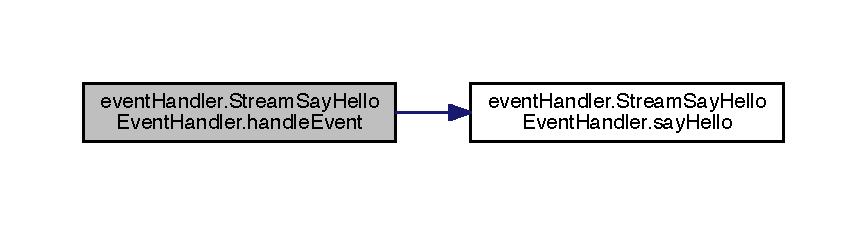
\includegraphics[width=350pt]{classevent_handler_1_1_stream_say_hello_event_handler_a859dc382ae8a35257af2149a9ed1c6b8_cgraph}
\end{center}
\end{figure}


\hypertarget{classevent_handler_1_1_stream_say_hello_event_handler_a6af4d6b8a6ed973d984a2eea55e405bc}{\index{event\+Handler\+::\+Stream\+Say\+Hello\+Event\+Handler@{event\+Handler\+::\+Stream\+Say\+Hello\+Event\+Handler}!say\+Hello@{say\+Hello}}
\index{say\+Hello@{say\+Hello}!event\+Handler\+::\+Stream\+Say\+Hello\+Event\+Handler@{event\+Handler\+::\+Stream\+Say\+Hello\+Event\+Handler}}
\subsubsection[{say\+Hello}]{\setlength{\rightskip}{0pt plus 5cm}void event\+Handler.\+Stream\+Say\+Hello\+Event\+Handler.\+say\+Hello (
\begin{DoxyParamCaption}
\item[{String\mbox{[}$\,$\mbox{]}}]{params}
\end{DoxyParamCaption}
)\hspace{0.3cm}{\ttfamily [private]}}}\label{classevent_handler_1_1_stream_say_hello_event_handler_a6af4d6b8a6ed973d984a2eea55e405bc}


Stream\+Say\+Hello\+Event\+Handler.\+java 파일의 49 번째 라인에서 정의되었습니다.


\begin{DoxyCode}
49                                            \{
50         \textcolor{comment}{//System.out.println("SayHello / NAME: " + params[0] + " / AGE: " + params[1]);}
51         \hyperlink{classevent_handler_1_1_stream_say_hello_event_handler_a9ce34e287f4621a4bd97e9b133e3a6f8}{logger}.fatal(\textcolor{stringliteral}{"SayHello / NAME: "} + params[0] + \textcolor{stringliteral}{" / AGE: "} + params[1]);
52     \}
\end{DoxyCode}


이 함수를 호출하는 함수들에 대한 그래프입니다.\+:\nopagebreak
\begin{figure}[H]
\begin{center}
\leavevmode
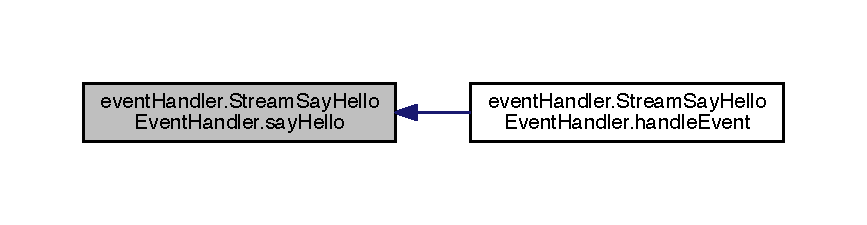
\includegraphics[width=350pt]{classevent_handler_1_1_stream_say_hello_event_handler_a6af4d6b8a6ed973d984a2eea55e405bc_icgraph}
\end{center}
\end{figure}




\subsection{멤버 데이타 문서화}
\hypertarget{classevent_handler_1_1_stream_say_hello_event_handler_a7caabf3a748346a2161f5b671eacc4b4}{\index{event\+Handler\+::\+Stream\+Say\+Hello\+Event\+Handler@{event\+Handler\+::\+Stream\+Say\+Hello\+Event\+Handler}!D\+A\+T\+A\+\_\+\+S\+I\+Z\+E@{D\+A\+T\+A\+\_\+\+S\+I\+Z\+E}}
\index{D\+A\+T\+A\+\_\+\+S\+I\+Z\+E@{D\+A\+T\+A\+\_\+\+S\+I\+Z\+E}!event\+Handler\+::\+Stream\+Say\+Hello\+Event\+Handler@{event\+Handler\+::\+Stream\+Say\+Hello\+Event\+Handler}}
\subsubsection[{D\+A\+T\+A\+\_\+\+S\+I\+Z\+E}]{\setlength{\rightskip}{0pt plus 5cm}final int event\+Handler.\+Stream\+Say\+Hello\+Event\+Handler.\+D\+A\+T\+A\+\_\+\+S\+I\+Z\+E = 512\hspace{0.3cm}{\ttfamily [static]}, {\ttfamily [private]}}}\label{classevent_handler_1_1_stream_say_hello_event_handler_a7caabf3a748346a2161f5b671eacc4b4}


Stream\+Say\+Hello\+Event\+Handler.\+java 파일의 18 번째 라인에서 정의되었습니다.

\hypertarget{classevent_handler_1_1_stream_say_hello_event_handler_a9ce34e287f4621a4bd97e9b133e3a6f8}{\index{event\+Handler\+::\+Stream\+Say\+Hello\+Event\+Handler@{event\+Handler\+::\+Stream\+Say\+Hello\+Event\+Handler}!logger@{logger}}
\index{logger@{logger}!event\+Handler\+::\+Stream\+Say\+Hello\+Event\+Handler@{event\+Handler\+::\+Stream\+Say\+Hello\+Event\+Handler}}
\subsubsection[{logger}]{\setlength{\rightskip}{0pt plus 5cm}Logger event\+Handler.\+Stream\+Say\+Hello\+Event\+Handler.\+logger = Logger.\+get\+Logger(Stream\+Say\+Hello\+Event\+Handler.\+class.\+get\+Name())\hspace{0.3cm}{\ttfamily [static]}, {\ttfamily [private]}}}\label{classevent_handler_1_1_stream_say_hello_event_handler_a9ce34e287f4621a4bd97e9b133e3a6f8}


Stream\+Say\+Hello\+Event\+Handler.\+java 파일의 16 번째 라인에서 정의되었습니다.

\hypertarget{classevent_handler_1_1_stream_say_hello_event_handler_af838acda55ea4de208e013ac0493364a}{\index{event\+Handler\+::\+Stream\+Say\+Hello\+Event\+Handler@{event\+Handler\+::\+Stream\+Say\+Hello\+Event\+Handler}!T\+O\+K\+E\+N\+\_\+\+N\+U\+M@{T\+O\+K\+E\+N\+\_\+\+N\+U\+M}}
\index{T\+O\+K\+E\+N\+\_\+\+N\+U\+M@{T\+O\+K\+E\+N\+\_\+\+N\+U\+M}!event\+Handler\+::\+Stream\+Say\+Hello\+Event\+Handler@{event\+Handler\+::\+Stream\+Say\+Hello\+Event\+Handler}}
\subsubsection[{T\+O\+K\+E\+N\+\_\+\+N\+U\+M}]{\setlength{\rightskip}{0pt plus 5cm}final int event\+Handler.\+Stream\+Say\+Hello\+Event\+Handler.\+T\+O\+K\+E\+N\+\_\+\+N\+U\+M = 2\hspace{0.3cm}{\ttfamily [static]}, {\ttfamily [private]}}}\label{classevent_handler_1_1_stream_say_hello_event_handler_af838acda55ea4de208e013ac0493364a}


Stream\+Say\+Hello\+Event\+Handler.\+java 파일의 19 번째 라인에서 정의되었습니다.



이 클래스에 대한 문서화 페이지는 다음의 파일로부터 생성되었습니다.\+:\begin{DoxyCompactItemize}
\item 
src/event\+Handler/\hyperlink{_stream_say_hello_event_handler_8java}{Stream\+Say\+Hello\+Event\+Handler.\+java}\end{DoxyCompactItemize}

\hypertarget{classevent_handler_1_1_stream_update_profile_event_handler}{\section{event\+Handler.\+Stream\+Update\+Profile\+Event\+Handler 클래스 참조}
\label{classevent_handler_1_1_stream_update_profile_event_handler}\index{event\+Handler.\+Stream\+Update\+Profile\+Event\+Handler@{event\+Handler.\+Stream\+Update\+Profile\+Event\+Handler}}
}


0x6001 헤더를 받았을 때 실행되는 event handler. \hyperlink{classevent_handler_1_1_stream_update_profile_event_handler_a888b80c6db463e195fe9ebefc39c721e}{update\+Profile()}를 갖고 있다.  




event\+Handler.\+Stream\+Update\+Profile\+Event\+Handler에 대한 상속 다이어그램 \+: 
\nopagebreak
\begin{figure}[H]
\begin{center}
\leavevmode
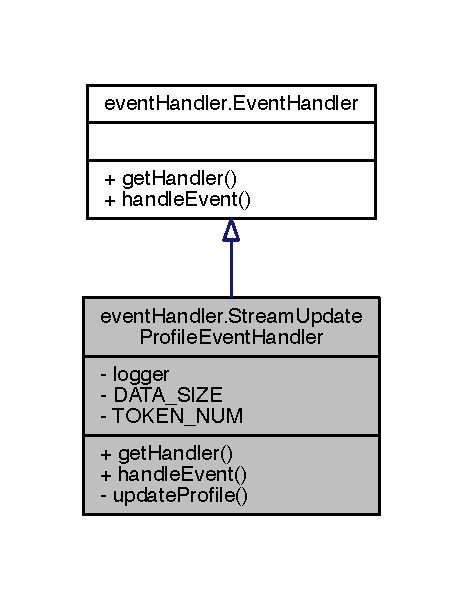
\includegraphics[width=222pt]{classevent_handler_1_1_stream_update_profile_event_handler__inherit__graph}
\end{center}
\end{figure}


event\+Handler.\+Stream\+Update\+Profile\+Event\+Handler에 대한 협력 다이어그램\+:
\nopagebreak
\begin{figure}[H]
\begin{center}
\leavevmode
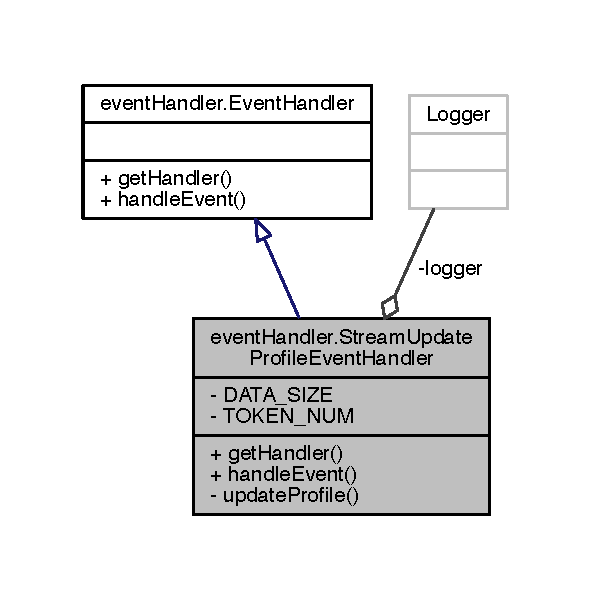
\includegraphics[width=283pt]{classevent_handler_1_1_stream_update_profile_event_handler__coll__graph}
\end{center}
\end{figure}
\subsection*{Public 멤버 함수}
\begin{DoxyCompactItemize}
\item 
String \hyperlink{classevent_handler_1_1_stream_update_profile_event_handler_a24bf455a312c225975d472516b4bb6f9}{get\+Handler} ()
\item 
void \hyperlink{classevent_handler_1_1_stream_update_profile_event_handler_a96b3a510c642a6848cff0afce54b7d8e}{handle\+Event} (Input\+Stream input\+Stream)
\end{DoxyCompactItemize}
\subsection*{Private 멤버 함수}
\begin{DoxyCompactItemize}
\item 
void \hyperlink{classevent_handler_1_1_stream_update_profile_event_handler_a888b80c6db463e195fe9ebefc39c721e}{update\+Profile} (String\mbox{[}$\,$\mbox{]} params)
\end{DoxyCompactItemize}
\subsection*{정적 Private 속성}
\begin{DoxyCompactItemize}
\item 
static Logger \hyperlink{classevent_handler_1_1_stream_update_profile_event_handler_a90754ca06692e3fc5767403f29a567b8}{logger} = Logger.\+get\+Logger(Stream\+Update\+Profile\+Event\+Handler.\+class.\+get\+Name())
\item 
static final int \hyperlink{classevent_handler_1_1_stream_update_profile_event_handler_a217e02fac4843d50927e5ebcb97baf0f}{D\+A\+T\+A\+\_\+\+S\+I\+Z\+E} = 1024
\item 
static final int \hyperlink{classevent_handler_1_1_stream_update_profile_event_handler_aeb1ccf4c9cc4e91dcb585e0c9bb3fbfe}{T\+O\+K\+E\+N\+\_\+\+N\+U\+M} = 5
\end{DoxyCompactItemize}


\subsection{상세한 설명}
0x6001 헤더를 받았을 때 실행되는 event handler. \hyperlink{classevent_handler_1_1_stream_update_profile_event_handler_a888b80c6db463e195fe9ebefc39c721e}{update\+Profile()}를 갖고 있다. 

\begin{DoxyDate}{날짜}
2014-\/09-\/24 
\end{DoxyDate}
\begin{DoxyAuthor}{작성자}
min 
\end{DoxyAuthor}


Stream\+Update\+Profile\+Event\+Handler.\+java 파일의 15 번째 라인에서 정의되었습니다.



\subsection{멤버 함수 문서화}
\hypertarget{classevent_handler_1_1_stream_update_profile_event_handler_a24bf455a312c225975d472516b4bb6f9}{\index{event\+Handler\+::\+Stream\+Update\+Profile\+Event\+Handler@{event\+Handler\+::\+Stream\+Update\+Profile\+Event\+Handler}!get\+Handler@{get\+Handler}}
\index{get\+Handler@{get\+Handler}!event\+Handler\+::\+Stream\+Update\+Profile\+Event\+Handler@{event\+Handler\+::\+Stream\+Update\+Profile\+Event\+Handler}}
\subsubsection[{get\+Handler}]{\setlength{\rightskip}{0pt plus 5cm}String event\+Handler.\+Stream\+Update\+Profile\+Event\+Handler.\+get\+Handler (
\begin{DoxyParamCaption}
{}
\end{DoxyParamCaption}
)}}\label{classevent_handler_1_1_stream_update_profile_event_handler_a24bf455a312c225975d472516b4bb6f9}


\hyperlink{interfaceevent_handler_1_1_event_handler_ada178635174014bad23584547462ac03}{event\+Handler.\+Event\+Handler}를 구현.



Stream\+Update\+Profile\+Event\+Handler.\+java 파일의 22 번째 라인에서 정의되었습니다.


\begin{DoxyCode}
22                                \{
23         \textcolor{keywordflow}{return} \textcolor{stringliteral}{"0x6001"};
24     \}
\end{DoxyCode}
\hypertarget{classevent_handler_1_1_stream_update_profile_event_handler_a96b3a510c642a6848cff0afce54b7d8e}{\index{event\+Handler\+::\+Stream\+Update\+Profile\+Event\+Handler@{event\+Handler\+::\+Stream\+Update\+Profile\+Event\+Handler}!handle\+Event@{handle\+Event}}
\index{handle\+Event@{handle\+Event}!event\+Handler\+::\+Stream\+Update\+Profile\+Event\+Handler@{event\+Handler\+::\+Stream\+Update\+Profile\+Event\+Handler}}
\subsubsection[{handle\+Event}]{\setlength{\rightskip}{0pt plus 5cm}void event\+Handler.\+Stream\+Update\+Profile\+Event\+Handler.\+handle\+Event (
\begin{DoxyParamCaption}
\item[{Input\+Stream}]{input\+Stream}
\end{DoxyParamCaption}
)}}\label{classevent_handler_1_1_stream_update_profile_event_handler_a96b3a510c642a6848cff0afce54b7d8e}


\hyperlink{interfaceevent_handler_1_1_event_handler_a4036ea3f27edd7df0caa57f42db27eed}{event\+Handler.\+Event\+Handler}를 구현.



Stream\+Update\+Profile\+Event\+Handler.\+java 파일의 26 번째 라인에서 정의되었습니다.


\begin{DoxyCode}
26                                                      \{
27         \textcolor{keywordflow}{try} \{
28             byte[] buffer = \textcolor{keyword}{new} byte[\hyperlink{classevent_handler_1_1_stream_update_profile_event_handler_a217e02fac4843d50927e5ebcb97baf0f}{DATA\_SIZE}];
29             inputStream.read(buffer);
30 
31             String data = \textcolor{keyword}{new} String(buffer);
32 
33             String[] params = \textcolor{keyword}{new} String[\hyperlink{classevent_handler_1_1_stream_update_profile_event_handler_aeb1ccf4c9cc4e91dcb585e0c9bb3fbfe}{TOKEN\_NUM}];
34             StringTokenizer token = \textcolor{keyword}{new} StringTokenizer(data, \textcolor{stringliteral}{"|"});
35 
36             \textcolor{keywordtype}{int} i = 0;
37             \textcolor{keywordflow}{while} (token.hasMoreTokens()) \{
38                 params[i] = token.nextToken();
39                 ++i;
40             \}
41 
42             \hyperlink{classevent_handler_1_1_stream_update_profile_event_handler_a888b80c6db463e195fe9ebefc39c721e}{updateProfile}(params);
43 
44         \} \textcolor{keywordflow}{catch} (IOException e) \{
45             e.printStackTrace();
46         \}
47     \}
\end{DoxyCode}


이 함수 내부에서 호출하는 함수들에 대한 그래프입니다.\+:\nopagebreak
\begin{figure}[H]
\begin{center}
\leavevmode
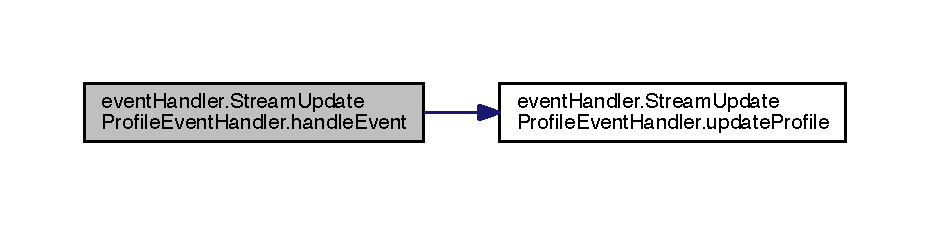
\includegraphics[width=350pt]{classevent_handler_1_1_stream_update_profile_event_handler_a96b3a510c642a6848cff0afce54b7d8e_cgraph}
\end{center}
\end{figure}


\hypertarget{classevent_handler_1_1_stream_update_profile_event_handler_a888b80c6db463e195fe9ebefc39c721e}{\index{event\+Handler\+::\+Stream\+Update\+Profile\+Event\+Handler@{event\+Handler\+::\+Stream\+Update\+Profile\+Event\+Handler}!update\+Profile@{update\+Profile}}
\index{update\+Profile@{update\+Profile}!event\+Handler\+::\+Stream\+Update\+Profile\+Event\+Handler@{event\+Handler\+::\+Stream\+Update\+Profile\+Event\+Handler}}
\subsubsection[{update\+Profile}]{\setlength{\rightskip}{0pt plus 5cm}void event\+Handler.\+Stream\+Update\+Profile\+Event\+Handler.\+update\+Profile (
\begin{DoxyParamCaption}
\item[{String\mbox{[}$\,$\mbox{]}}]{params}
\end{DoxyParamCaption}
)\hspace{0.3cm}{\ttfamily [private]}}}\label{classevent_handler_1_1_stream_update_profile_event_handler_a888b80c6db463e195fe9ebefc39c721e}


Stream\+Update\+Profile\+Event\+Handler.\+java 파일의 49 번째 라인에서 정의되었습니다.


\begin{DoxyCode}
49                                                 \{
50         \textcolor{comment}{//System.out.println("UpdateProfile / " + "ID: " + params[0] + " / " + "PASSWORD: " + params[1] + "
       / "}
51         \textcolor{comment}{//      + "NAME: " + params[2] + " / " + "AGE: " + params[3] + " / " + "GENDER: " + params[4]);}
52         
53         \hyperlink{classevent_handler_1_1_stream_update_profile_event_handler_a90754ca06692e3fc5767403f29a567b8}{logger}.fatal(\textcolor{stringliteral}{"UpdateProfile / "} + \textcolor{stringliteral}{"ID: "} + params[0] + \textcolor{stringliteral}{" / "} + \textcolor{stringliteral}{"PASSWORD: "} + params[1] + \textcolor{stringliteral}{" /
       "}
54                 + \textcolor{stringliteral}{"NAME: "} + params[2] + \textcolor{stringliteral}{" / "} + \textcolor{stringliteral}{"AGE: "} + params[3] + \textcolor{stringliteral}{" / "} + \textcolor{stringliteral}{"GENDER: "} + params[4]);
55     \}
\end{DoxyCode}


이 함수를 호출하는 함수들에 대한 그래프입니다.\+:\nopagebreak
\begin{figure}[H]
\begin{center}
\leavevmode
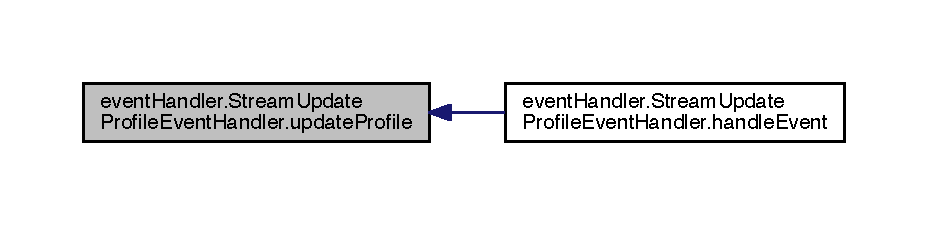
\includegraphics[width=350pt]{classevent_handler_1_1_stream_update_profile_event_handler_a888b80c6db463e195fe9ebefc39c721e_icgraph}
\end{center}
\end{figure}




\subsection{멤버 데이타 문서화}
\hypertarget{classevent_handler_1_1_stream_update_profile_event_handler_a217e02fac4843d50927e5ebcb97baf0f}{\index{event\+Handler\+::\+Stream\+Update\+Profile\+Event\+Handler@{event\+Handler\+::\+Stream\+Update\+Profile\+Event\+Handler}!D\+A\+T\+A\+\_\+\+S\+I\+Z\+E@{D\+A\+T\+A\+\_\+\+S\+I\+Z\+E}}
\index{D\+A\+T\+A\+\_\+\+S\+I\+Z\+E@{D\+A\+T\+A\+\_\+\+S\+I\+Z\+E}!event\+Handler\+::\+Stream\+Update\+Profile\+Event\+Handler@{event\+Handler\+::\+Stream\+Update\+Profile\+Event\+Handler}}
\subsubsection[{D\+A\+T\+A\+\_\+\+S\+I\+Z\+E}]{\setlength{\rightskip}{0pt plus 5cm}final int event\+Handler.\+Stream\+Update\+Profile\+Event\+Handler.\+D\+A\+T\+A\+\_\+\+S\+I\+Z\+E = 1024\hspace{0.3cm}{\ttfamily [static]}, {\ttfamily [private]}}}\label{classevent_handler_1_1_stream_update_profile_event_handler_a217e02fac4843d50927e5ebcb97baf0f}


Stream\+Update\+Profile\+Event\+Handler.\+java 파일의 18 번째 라인에서 정의되었습니다.

\hypertarget{classevent_handler_1_1_stream_update_profile_event_handler_a90754ca06692e3fc5767403f29a567b8}{\index{event\+Handler\+::\+Stream\+Update\+Profile\+Event\+Handler@{event\+Handler\+::\+Stream\+Update\+Profile\+Event\+Handler}!logger@{logger}}
\index{logger@{logger}!event\+Handler\+::\+Stream\+Update\+Profile\+Event\+Handler@{event\+Handler\+::\+Stream\+Update\+Profile\+Event\+Handler}}
\subsubsection[{logger}]{\setlength{\rightskip}{0pt plus 5cm}Logger event\+Handler.\+Stream\+Update\+Profile\+Event\+Handler.\+logger = Logger.\+get\+Logger(Stream\+Update\+Profile\+Event\+Handler.\+class.\+get\+Name())\hspace{0.3cm}{\ttfamily [static]}, {\ttfamily [private]}}}\label{classevent_handler_1_1_stream_update_profile_event_handler_a90754ca06692e3fc5767403f29a567b8}


Stream\+Update\+Profile\+Event\+Handler.\+java 파일의 16 번째 라인에서 정의되었습니다.

\hypertarget{classevent_handler_1_1_stream_update_profile_event_handler_aeb1ccf4c9cc4e91dcb585e0c9bb3fbfe}{\index{event\+Handler\+::\+Stream\+Update\+Profile\+Event\+Handler@{event\+Handler\+::\+Stream\+Update\+Profile\+Event\+Handler}!T\+O\+K\+E\+N\+\_\+\+N\+U\+M@{T\+O\+K\+E\+N\+\_\+\+N\+U\+M}}
\index{T\+O\+K\+E\+N\+\_\+\+N\+U\+M@{T\+O\+K\+E\+N\+\_\+\+N\+U\+M}!event\+Handler\+::\+Stream\+Update\+Profile\+Event\+Handler@{event\+Handler\+::\+Stream\+Update\+Profile\+Event\+Handler}}
\subsubsection[{T\+O\+K\+E\+N\+\_\+\+N\+U\+M}]{\setlength{\rightskip}{0pt plus 5cm}final int event\+Handler.\+Stream\+Update\+Profile\+Event\+Handler.\+T\+O\+K\+E\+N\+\_\+\+N\+U\+M = 5\hspace{0.3cm}{\ttfamily [static]}, {\ttfamily [private]}}}\label{classevent_handler_1_1_stream_update_profile_event_handler_aeb1ccf4c9cc4e91dcb585e0c9bb3fbfe}


Stream\+Update\+Profile\+Event\+Handler.\+java 파일의 19 번째 라인에서 정의되었습니다.



이 클래스에 대한 문서화 페이지는 다음의 파일로부터 생성되었습니다.\+:\begin{DoxyCompactItemize}
\item 
src/event\+Handler/\hyperlink{_stream_update_profile_event_handler_8java}{Stream\+Update\+Profile\+Event\+Handler.\+java}\end{DoxyCompactItemize}

\hypertarget{classbasic_server_1_1_thread_per_dispatcher}{\section{basic\+Server.\+Thread\+Per\+Dispatcher 클래스 참조}
\label{classbasic_server_1_1_thread_per_dispatcher}\index{basic\+Server.\+Thread\+Per\+Dispatcher@{basic\+Server.\+Thread\+Per\+Dispatcher}}
}


single thread dispatcher. Demultiplexer를 실행시킨다.  




basic\+Server.\+Thread\+Per\+Dispatcher에 대한 상속 다이어그램 \+: 
\nopagebreak
\begin{figure}[H]
\begin{center}
\leavevmode
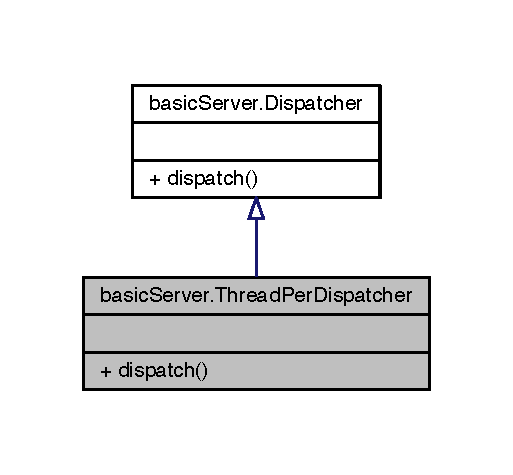
\includegraphics[width=246pt]{classbasic_server_1_1_thread_per_dispatcher__inherit__graph}
\end{center}
\end{figure}


basic\+Server.\+Thread\+Per\+Dispatcher에 대한 협력 다이어그램\+:
\nopagebreak
\begin{figure}[H]
\begin{center}
\leavevmode
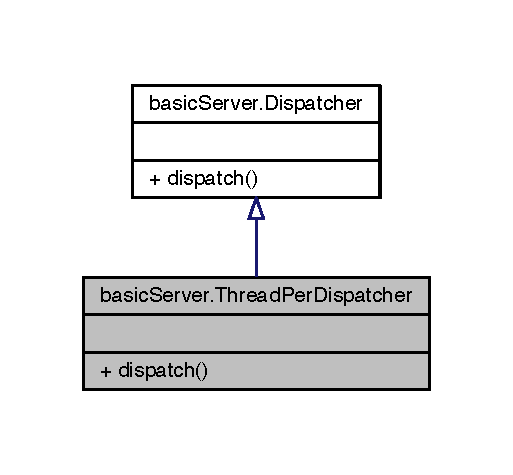
\includegraphics[width=246pt]{classbasic_server_1_1_thread_per_dispatcher__coll__graph}
\end{center}
\end{figure}
\subsection*{Public 멤버 함수}
\begin{DoxyCompactItemize}
\item 
void \hyperlink{classbasic_server_1_1_thread_per_dispatcher_af7be4592fa9f81c011985b4e0c0c3b2a}{dispatch} (Server\+Socket server\+Socket, \hyperlink{classbasic_server_1_1_handle_map}{Handle\+Map} handle\+Map)
\end{DoxyCompactItemize}


\subsection{상세한 설명}
single thread dispatcher. Demultiplexer를 실행시킨다. 

\begin{DoxyDate}{날짜}
2014-\/09-\/24 
\end{DoxyDate}
\begin{DoxyAuthor}{작성자}
min 
\end{DoxyAuthor}


Thread\+Per\+Dispatcher.\+java 파일의 13 번째 라인에서 정의되었습니다.



\subsection{멤버 함수 문서화}
\hypertarget{classbasic_server_1_1_thread_per_dispatcher_af7be4592fa9f81c011985b4e0c0c3b2a}{\index{basic\+Server\+::\+Thread\+Per\+Dispatcher@{basic\+Server\+::\+Thread\+Per\+Dispatcher}!dispatch@{dispatch}}
\index{dispatch@{dispatch}!basic\+Server\+::\+Thread\+Per\+Dispatcher@{basic\+Server\+::\+Thread\+Per\+Dispatcher}}
\subsubsection[{dispatch}]{\setlength{\rightskip}{0pt plus 5cm}void basic\+Server.\+Thread\+Per\+Dispatcher.\+dispatch (
\begin{DoxyParamCaption}
\item[{Server\+Socket}]{server\+Socket, }
\item[{{\bf Handle\+Map}}]{handle\+Map}
\end{DoxyParamCaption}
)}}\label{classbasic_server_1_1_thread_per_dispatcher_af7be4592fa9f81c011985b4e0c0c3b2a}


\hyperlink{interfacebasic_server_1_1_dispatcher_a9a8d3e47b27a6161f8f39bf63fa9e198}{basic\+Server.\+Dispatcher}를 구현.



Thread\+Per\+Dispatcher.\+java 파일의 15 번째 라인에서 정의되었습니다.


\begin{DoxyCode}
15                                                                          \{
16         \textcolor{keywordflow}{while} (\textcolor{keyword}{true}) \{
17             \textcolor{keywordflow}{try} \{
18                 Socket socket = serverSocket.accept();
19 
20                 Demultiplexer demultiplexer = \textcolor{keyword}{new} Demultiplexer(socket, handleMap);
21                 Thread thread = \textcolor{keyword}{new} Thread(demultiplexer);
22 
23                 thread.start();
24             \} \textcolor{keywordflow}{catch} (IOException e) \{
25                 e.printStackTrace();
26             \}
27         \}
28     \}
\end{DoxyCode}


이 클래스에 대한 문서화 페이지는 다음의 파일로부터 생성되었습니다.\+:\begin{DoxyCompactItemize}
\item 
src/basic\+Server/\hyperlink{_thread_per_dispatcher_8java}{Thread\+Per\+Dispatcher.\+java}\end{DoxyCompactItemize}

\hypertarget{classbasic_server_1_1_thread_pool_dispatcher}{\section{basic\+Server.\+Thread\+Pool\+Dispatcher 클래스 참조}
\label{classbasic_server_1_1_thread_pool_dispatcher}\index{basic\+Server.\+Thread\+Pool\+Dispatcher@{basic\+Server.\+Thread\+Pool\+Dispatcher}}
}


basic\+Server.\+Thread\+Pool\+Dispatcher에 대한 상속 다이어그램 \+: 
\nopagebreak
\begin{figure}[H]
\begin{center}
\leavevmode
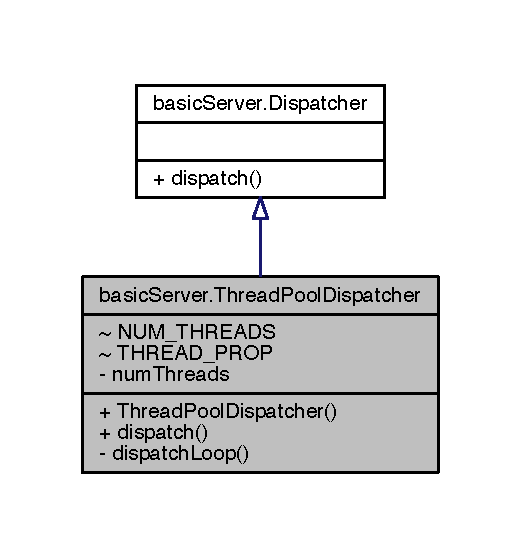
\includegraphics[width=250pt]{classbasic_server_1_1_thread_pool_dispatcher__inherit__graph}
\end{center}
\end{figure}


basic\+Server.\+Thread\+Pool\+Dispatcher에 대한 협력 다이어그램\+:
\nopagebreak
\begin{figure}[H]
\begin{center}
\leavevmode
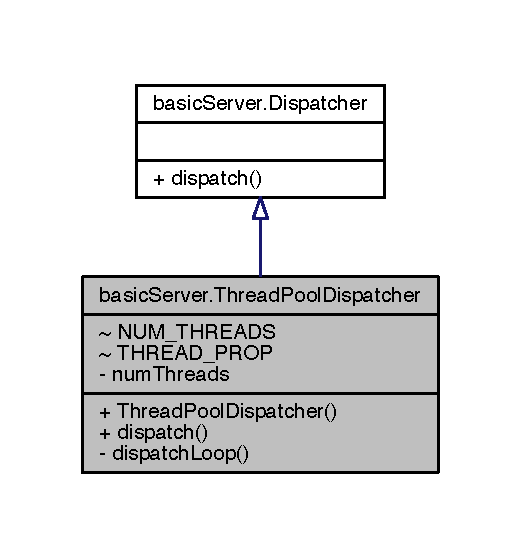
\includegraphics[width=250pt]{classbasic_server_1_1_thread_pool_dispatcher__coll__graph}
\end{center}
\end{figure}
\subsection*{Public 멤버 함수}
\begin{DoxyCompactItemize}
\item 
\hyperlink{classbasic_server_1_1_thread_pool_dispatcher_a26fda3271602b19753ce6e2d6d9b308a}{Thread\+Pool\+Dispatcher} ()
\item 
void \hyperlink{classbasic_server_1_1_thread_pool_dispatcher_a5311a036b85df65c640d955f253ecc83}{dispatch} (final Server\+Socket server\+Socket, final \hyperlink{classbasic_server_1_1_handle_map}{Handle\+Map} handle\+Map)
\item 
void \hyperlink{interfacebasic_server_1_1_dispatcher_a9a8d3e47b27a6161f8f39bf63fa9e198}{dispatch} (Server\+Socket server\+Socket, \hyperlink{classbasic_server_1_1_handle_map}{Handle\+Map} handle\+Map)
\end{DoxyCompactItemize}
\subsection*{Private 멤버 함수}
\begin{DoxyCompactItemize}
\item 
void \hyperlink{classbasic_server_1_1_thread_pool_dispatcher_a80411d17546dd5ff40af166ef50e2e32}{dispatch\+Loop} (Server\+Socket server\+Socket, \hyperlink{classbasic_server_1_1_handle_map}{Handle\+Map} handle\+Map)
\end{DoxyCompactItemize}
\subsection*{Private 속성}
\begin{DoxyCompactItemize}
\item 
int \hyperlink{classbasic_server_1_1_thread_pool_dispatcher_a0c78b67cc799e2aa23038d96e9bf9af8}{num\+Threads}
\end{DoxyCompactItemize}


\subsection{상세한 설명}


Thread\+Pool\+Dispatcher.\+java 파일의 13 번째 라인에서 정의되었습니다.



\subsection{생성자 \& 소멸자 문서화}
\hypertarget{classbasic_server_1_1_thread_pool_dispatcher_a26fda3271602b19753ce6e2d6d9b308a}{\index{basic\+Server\+::\+Thread\+Pool\+Dispatcher@{basic\+Server\+::\+Thread\+Pool\+Dispatcher}!Thread\+Pool\+Dispatcher@{Thread\+Pool\+Dispatcher}}
\index{Thread\+Pool\+Dispatcher@{Thread\+Pool\+Dispatcher}!basic\+Server\+::\+Thread\+Pool\+Dispatcher@{basic\+Server\+::\+Thread\+Pool\+Dispatcher}}
\subsubsection[{Thread\+Pool\+Dispatcher}]{\setlength{\rightskip}{0pt plus 5cm}basic\+Server.\+Thread\+Pool\+Dispatcher.\+Thread\+Pool\+Dispatcher (
\begin{DoxyParamCaption}
{}
\end{DoxyParamCaption}
)}}\label{classbasic_server_1_1_thread_pool_dispatcher_a26fda3271602b19753ce6e2d6d9b308a}


Thread\+Pool\+Dispatcher.\+java 파일의 20 번째 라인에서 정의되었습니다.


\begin{DoxyCode}
20                                   \{
21         \textcolor{comment}{// 시스템 정보의 스레드 개수를 가져오거나, 없으면 우리가 설정한 값을 사용함}
22         \hyperlink{classbasic_server_1_1_thread_pool_dispatcher_a0c78b67cc799e2aa23038d96e9bf9af8}{numThreads} = Integer.parseInt(System.getProperty(THREAD\_PROP, NUM\_THREADS));
23     \}
\end{DoxyCode}


\subsection{멤버 함수 문서화}
\hypertarget{interfacebasic_server_1_1_dispatcher_a9a8d3e47b27a6161f8f39bf63fa9e198}{\index{basic\+Server\+::\+Thread\+Pool\+Dispatcher@{basic\+Server\+::\+Thread\+Pool\+Dispatcher}!dispatch@{dispatch}}
\index{dispatch@{dispatch}!basic\+Server\+::\+Thread\+Pool\+Dispatcher@{basic\+Server\+::\+Thread\+Pool\+Dispatcher}}
\subsubsection[{dispatch}]{\setlength{\rightskip}{0pt plus 5cm}void basic\+Server.\+Dispatcher.\+dispatch (
\begin{DoxyParamCaption}
\item[{Server\+Socket}]{server\+Socket, }
\item[{{\bf Handle\+Map}}]{handle\+Map}
\end{DoxyParamCaption}
)\hspace{0.3cm}{\ttfamily [inherited]}}}\label{interfacebasic_server_1_1_dispatcher_a9a8d3e47b27a6161f8f39bf63fa9e198}


\hyperlink{classbasic_server_1_1_thread_per_dispatcher_af7be4592fa9f81c011985b4e0c0c3b2a}{basic\+Server.\+Thread\+Per\+Dispatcher}에서 구현되었습니다.

\hypertarget{classbasic_server_1_1_thread_pool_dispatcher_a5311a036b85df65c640d955f253ecc83}{\index{basic\+Server\+::\+Thread\+Pool\+Dispatcher@{basic\+Server\+::\+Thread\+Pool\+Dispatcher}!dispatch@{dispatch}}
\index{dispatch@{dispatch}!basic\+Server\+::\+Thread\+Pool\+Dispatcher@{basic\+Server\+::\+Thread\+Pool\+Dispatcher}}
\subsubsection[{dispatch}]{\setlength{\rightskip}{0pt plus 5cm}void basic\+Server.\+Thread\+Pool\+Dispatcher.\+dispatch (
\begin{DoxyParamCaption}
\item[{final Server\+Socket}]{server\+Socket, }
\item[{final {\bf Handle\+Map}}]{handle\+Map}
\end{DoxyParamCaption}
)}}\label{classbasic_server_1_1_thread_pool_dispatcher_a5311a036b85df65c640d955f253ecc83}


Thread\+Pool\+Dispatcher.\+java 파일의 26 번째 라인에서 정의되었습니다.


\begin{DoxyCode}
26                                                                                      \{
27         \textcolor{keywordflow}{for} (\textcolor{keywordtype}{int} idx\_thread = 0; idx\_thread < (\hyperlink{classbasic_server_1_1_thread_pool_dispatcher_a0c78b67cc799e2aa23038d96e9bf9af8}{numThreads} - 1); idx\_thread++) \{
28             Thread thread = \textcolor{keyword}{new} Thread() \{
29                 \textcolor{keyword}{public} \textcolor{keywordtype}{void} run() \{
30                     \hyperlink{classbasic_server_1_1_thread_pool_dispatcher_a80411d17546dd5ff40af166ef50e2e32}{dispatchLoop}(serverSocket, handleMap);
31                 \}
32             \};
33             thread.start();
34             
35             System.out.println(\textcolor{stringliteral}{"CREATE / START Thread: "} + thread.getName());
36         \}
37         System.out.println(\textcolor{stringliteral}{"INTERATIVE SERVER STARTED IN MAIN THREAD: "} + Thread.currentThread().getName())
      ;
38         
39         \hyperlink{classbasic_server_1_1_thread_pool_dispatcher_a80411d17546dd5ff40af166ef50e2e32}{dispatchLoop}(serverSocket, handleMap);
40     \}
\end{DoxyCode}


이 함수 내부에서 호출하는 함수들에 대한 그래프입니다.\+:\nopagebreak
\begin{figure}[H]
\begin{center}
\leavevmode
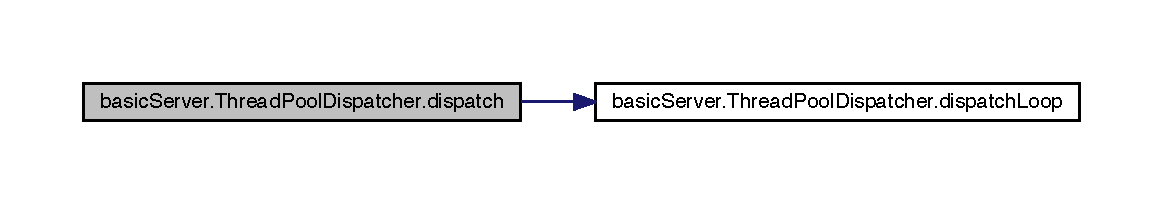
\includegraphics[width=350pt]{classbasic_server_1_1_thread_pool_dispatcher_a5311a036b85df65c640d955f253ecc83_cgraph}
\end{center}
\end{figure}




이 함수를 호출하는 함수들에 대한 그래프입니다.\+:\nopagebreak
\begin{figure}[H]
\begin{center}
\leavevmode
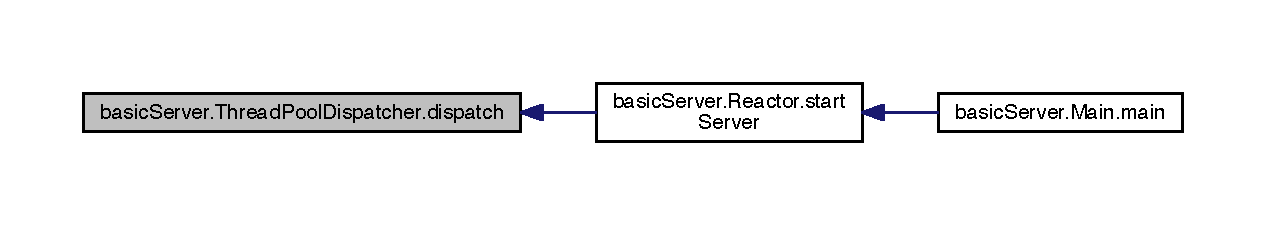
\includegraphics[width=350pt]{classbasic_server_1_1_thread_pool_dispatcher_a5311a036b85df65c640d955f253ecc83_icgraph}
\end{center}
\end{figure}


\hypertarget{classbasic_server_1_1_thread_pool_dispatcher_a80411d17546dd5ff40af166ef50e2e32}{\index{basic\+Server\+::\+Thread\+Pool\+Dispatcher@{basic\+Server\+::\+Thread\+Pool\+Dispatcher}!dispatch\+Loop@{dispatch\+Loop}}
\index{dispatch\+Loop@{dispatch\+Loop}!basic\+Server\+::\+Thread\+Pool\+Dispatcher@{basic\+Server\+::\+Thread\+Pool\+Dispatcher}}
\subsubsection[{dispatch\+Loop}]{\setlength{\rightskip}{0pt plus 5cm}void basic\+Server.\+Thread\+Pool\+Dispatcher.\+dispatch\+Loop (
\begin{DoxyParamCaption}
\item[{Server\+Socket}]{server\+Socket, }
\item[{{\bf Handle\+Map}}]{handle\+Map}
\end{DoxyParamCaption}
)\hspace{0.3cm}{\ttfamily [private]}}}\label{classbasic_server_1_1_thread_pool_dispatcher_a80411d17546dd5ff40af166ef50e2e32}


Thread\+Pool\+Dispatcher.\+java 파일의 42 번째 라인에서 정의되었습니다.


\begin{DoxyCode}
42                                                                               \{
43         \textcolor{keywordflow}{while} (\textcolor{keyword}{true}) \{
44             \textcolor{keywordflow}{try} \{
45                 Socket socket = serverSocket.accept();
46 
47                 Demultiplexer demultiplexer = \textcolor{keyword}{new} Demultiplexer(socket, handleMap);
48                 Thread thread = \textcolor{keyword}{new} Thread(demultiplexer);
49 
50                 thread.start();
51             \} \textcolor{keywordflow}{catch} (IOException e) \{
52                 e.printStackTrace();
53             \}
54         \}
55     \}
\end{DoxyCode}


이 함수를 호출하는 함수들에 대한 그래프입니다.\+:\nopagebreak
\begin{figure}[H]
\begin{center}
\leavevmode
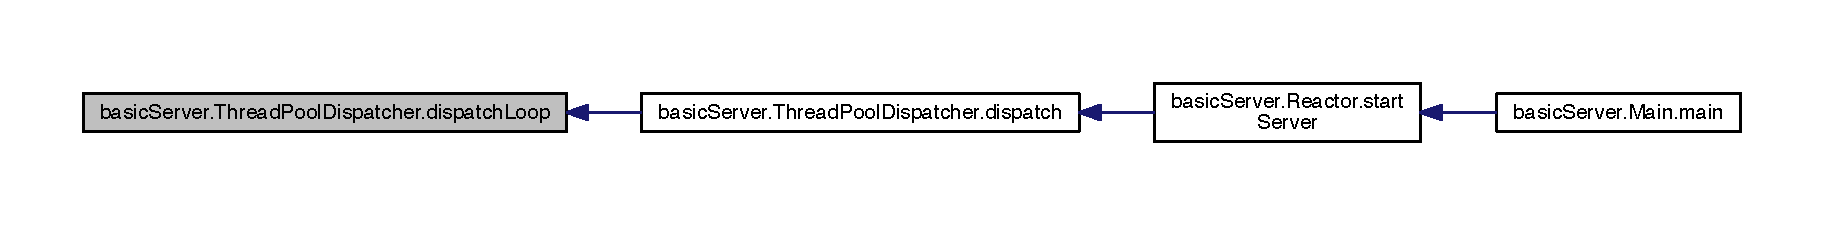
\includegraphics[width=350pt]{classbasic_server_1_1_thread_pool_dispatcher_a80411d17546dd5ff40af166ef50e2e32_icgraph}
\end{center}
\end{figure}




\subsection{멤버 데이타 문서화}
\hypertarget{classbasic_server_1_1_thread_pool_dispatcher_a0c78b67cc799e2aa23038d96e9bf9af8}{\index{basic\+Server\+::\+Thread\+Pool\+Dispatcher@{basic\+Server\+::\+Thread\+Pool\+Dispatcher}!num\+Threads@{num\+Threads}}
\index{num\+Threads@{num\+Threads}!basic\+Server\+::\+Thread\+Pool\+Dispatcher@{basic\+Server\+::\+Thread\+Pool\+Dispatcher}}
\subsubsection[{num\+Threads}]{\setlength{\rightskip}{0pt plus 5cm}int basic\+Server.\+Thread\+Pool\+Dispatcher.\+num\+Threads\hspace{0.3cm}{\ttfamily [private]}}}\label{classbasic_server_1_1_thread_pool_dispatcher_a0c78b67cc799e2aa23038d96e9bf9af8}


Thread\+Pool\+Dispatcher.\+java 파일의 18 번째 라인에서 정의되었습니다.



이 클래스에 대한 문서화 페이지는 다음의 파일로부터 생성되었습니다.\+:\begin{DoxyCompactItemize}
\item 
src/basic\+Server/\hyperlink{_thread_pool_dispatcher_8java}{Thread\+Pool\+Dispatcher.\+java}\end{DoxyCompactItemize}

\chapter{파일 문서화}
\hypertarget{_demultiplexer_8java}{\section{src/basic\+Server/\+Demultiplexer.java 파일 참조}
\label{_demultiplexer_8java}\index{src/basic\+Server/\+Demultiplexer.\+java@{src/basic\+Server/\+Demultiplexer.\+java}}
}
\subsection*{클래스}
\begin{DoxyCompactItemize}
\item 
class \hyperlink{classbasic_server_1_1_demultiplexer}{basic\+Server.\+Demultiplexer}
\begin{DoxyCompactList}\small\item\em Input Stream에서 header를 읽고 적절한 event handler를 부른다. \end{DoxyCompactList}\end{DoxyCompactItemize}
\subsection*{패키지}
\begin{DoxyCompactItemize}
\item 
package \hyperlink{namespacebasic_server}{basic\+Server}
\end{DoxyCompactItemize}

\hypertarget{_dispatcher_8java}{\section{src/basic\+Server/\+Dispatcher.java 파일 참조}
\label{_dispatcher_8java}\index{src/basic\+Server/\+Dispatcher.\+java@{src/basic\+Server/\+Dispatcher.\+java}}
}
\subsection*{클래스}
\begin{DoxyCompactItemize}
\item 
interface \hyperlink{interfacebasic_server_1_1_dispatcher}{basic\+Server.\+Dispatcher}
\begin{DoxyCompactList}\small\item\em dispatcher의 D\+I를 위한 인터페이스 \end{DoxyCompactList}\end{DoxyCompactItemize}
\subsection*{패키지}
\begin{DoxyCompactItemize}
\item 
package \hyperlink{namespacebasic_server}{basic\+Server}
\end{DoxyCompactItemize}

\hypertarget{_handle_map_8java}{\section{src/basic\+Server/\+Handle\+Map.java 파일 참조}
\label{_handle_map_8java}\index{src/basic\+Server/\+Handle\+Map.\+java@{src/basic\+Server/\+Handle\+Map.\+java}}
}
\subsection*{클래스}
\begin{DoxyCompactItemize}
\item 
class \hyperlink{classbasic_server_1_1_handle_map}{basic\+Server.\+Handle\+Map}
\begin{DoxyCompactList}\small\item\em header와 그에 대응하는 event handler를 기억함 \end{DoxyCompactList}\end{DoxyCompactItemize}
\subsection*{패키지}
\begin{DoxyCompactItemize}
\item 
package \hyperlink{namespacebasic_server}{basic\+Server}
\end{DoxyCompactItemize}

\hypertarget{_main_8java}{\section{src/basic\+Server/\+Main.java 파일 참조}
\label{_main_8java}\index{src/basic\+Server/\+Main.\+java@{src/basic\+Server/\+Main.\+java}}
}
\subsection*{클래스}
\begin{DoxyCompactItemize}
\item 
class \hyperlink{classbasic_server_1_1_main}{basic\+Server.\+Main}
\begin{DoxyCompactList}\small\item\em main함수를 갖고 있다. reactor를 new하고 실행시킨다. \end{DoxyCompactList}\end{DoxyCompactItemize}
\subsection*{패키지}
\begin{DoxyCompactItemize}
\item 
package \hyperlink{namespacebasic_server}{basic\+Server}
\end{DoxyCompactItemize}

\hypertarget{_reactor_8java}{\section{src/basic\+Server/\+Reactor.java 파일 참조}
\label{_reactor_8java}\index{src/basic\+Server/\+Reactor.\+java@{src/basic\+Server/\+Reactor.\+java}}
}
\subsection*{클래스}
\begin{DoxyCompactItemize}
\item 
class \hyperlink{classbasic_server_1_1_reactor}{basic\+Server.\+Reactor}
\begin{DoxyCompactList}\small\item\em dispatcher 관리, header와 대응되는 event handler를 관리. \end{DoxyCompactList}\end{DoxyCompactItemize}
\subsection*{패키지}
\begin{DoxyCompactItemize}
\item 
package \hyperlink{namespacebasic_server}{basic\+Server}
\end{DoxyCompactItemize}

\hypertarget{_thread_per_dispatcher_8java}{\section{src/basic\+Server/\+Thread\+Per\+Dispatcher.java 파일 참조}
\label{_thread_per_dispatcher_8java}\index{src/basic\+Server/\+Thread\+Per\+Dispatcher.\+java@{src/basic\+Server/\+Thread\+Per\+Dispatcher.\+java}}
}
\subsection*{클래스}
\begin{DoxyCompactItemize}
\item 
class \hyperlink{classbasic_server_1_1_thread_per_dispatcher}{basic\+Server.\+Thread\+Per\+Dispatcher}
\begin{DoxyCompactList}\small\item\em single thread dispatcher. Demultiplexer를 실행시킨다. \end{DoxyCompactList}\end{DoxyCompactItemize}
\subsection*{패키지}
\begin{DoxyCompactItemize}
\item 
package \hyperlink{namespacebasic_server}{basic\+Server}
\end{DoxyCompactItemize}

\hypertarget{_thread_pool_dispatcher_8java}{\section{src/basic\+Server/\+Thread\+Pool\+Dispatcher.java 파일 참조}
\label{_thread_pool_dispatcher_8java}\index{src/basic\+Server/\+Thread\+Pool\+Dispatcher.\+java@{src/basic\+Server/\+Thread\+Pool\+Dispatcher.\+java}}
}
\subsection*{클래스}
\begin{DoxyCompactItemize}
\item 
class \hyperlink{classbasic_server_1_1_thread_pool_dispatcher}{basic\+Server.\+Thread\+Pool\+Dispatcher}
\end{DoxyCompactItemize}
\subsection*{패키지}
\begin{DoxyCompactItemize}
\item 
package \hyperlink{namespacebasic_server}{basic\+Server}
\end{DoxyCompactItemize}

\hypertarget{_event_handler_8java}{\section{src/event\+Handler/\+Event\+Handler.java 파일 참조}
\label{_event_handler_8java}\index{src/event\+Handler/\+Event\+Handler.\+java@{src/event\+Handler/\+Event\+Handler.\+java}}
}
\subsection*{클래스}
\begin{DoxyCompactItemize}
\item 
interface \hyperlink{interfaceevent_handler_1_1_event_handler}{event\+Handler.\+Event\+Handler}
\begin{DoxyCompactList}\small\item\em event handler의 메소드를 정의한 interface. \end{DoxyCompactList}\end{DoxyCompactItemize}
\subsection*{패키지}
\begin{DoxyCompactItemize}
\item 
package \hyperlink{namespaceevent_handler}{event\+Handler}
\end{DoxyCompactItemize}

\hypertarget{_stream_say_hello_event_handler_8java}{\section{src/event\+Handler/\+Stream\+Say\+Hello\+Event\+Handler.java 파일 참조}
\label{_stream_say_hello_event_handler_8java}\index{src/event\+Handler/\+Stream\+Say\+Hello\+Event\+Handler.\+java@{src/event\+Handler/\+Stream\+Say\+Hello\+Event\+Handler.\+java}}
}
\subsection*{클래스}
\begin{DoxyCompactItemize}
\item 
class \hyperlink{classevent_handler_1_1_stream_say_hello_event_handler}{event\+Handler.\+Stream\+Say\+Hello\+Event\+Handler}
\begin{DoxyCompactList}\small\item\em 0x5001 헤더를 받았을 때 실행되는 event handler. \hyperlink{classevent_handler_1_1_stream_say_hello_event_handler_a6af4d6b8a6ed973d984a2eea55e405bc}{say\+Hello()}를 갖고 있다. \end{DoxyCompactList}\end{DoxyCompactItemize}
\subsection*{패키지}
\begin{DoxyCompactItemize}
\item 
package \hyperlink{namespaceevent_handler}{event\+Handler}
\end{DoxyCompactItemize}

\hypertarget{_stream_update_profile_event_handler_8java}{\section{src/event\+Handler/\+Stream\+Update\+Profile\+Event\+Handler.java 파일 참조}
\label{_stream_update_profile_event_handler_8java}\index{src/event\+Handler/\+Stream\+Update\+Profile\+Event\+Handler.\+java@{src/event\+Handler/\+Stream\+Update\+Profile\+Event\+Handler.\+java}}
}
\subsection*{클래스}
\begin{DoxyCompactItemize}
\item 
class \hyperlink{classevent_handler_1_1_stream_update_profile_event_handler}{event\+Handler.\+Stream\+Update\+Profile\+Event\+Handler}
\begin{DoxyCompactList}\small\item\em 0x6001 헤더를 받았을 때 실행되는 event handler. \hyperlink{classevent_handler_1_1_stream_update_profile_event_handler_a888b80c6db463e195fe9ebefc39c721e}{update\+Profile()}를 갖고 있다. \end{DoxyCompactList}\end{DoxyCompactItemize}
\subsection*{패키지}
\begin{DoxyCompactItemize}
\item 
package \hyperlink{namespaceevent_handler}{event\+Handler}
\end{DoxyCompactItemize}

%--- End generated contents ---

% Index
\newpage
\phantomsection
\addcontentsline{toc}{chapter}{색인}
\printindex

\end{document}
